%to have line numbers
%\RequirePackage{lineno}
\documentclass[10pt, letterpaper]{article}      
\usepackage[margin=.1cm,font=small,labelfont=bf]{caption}[2007/03/09]
%\usepackage{endnotes}
%\let\footnote=\endnote
\usepackage{setspace}
\usepackage{longtable}                        
\usepackage{anysize}                          
\usepackage{natbib}                           
%\bibpunct{(}{)}{,}{a}{,}{,}                   
\bibpunct{(}{)}{,}{a}{}{,}                   
\usepackage{amsmath}
\usepackage[% draft,
pdftex]{graphicx} %draft is a way to exclude figures                
\usepackage{epstopdf}
\usepackage{hyperref}                             % For creating hyperlinks in cross references
\hypersetup{pdfborder={0 0 0.4}} %have nice light boxes on refs

% \usepackage[margins]{trackchanges}

% \note[editor]{The note}
% \annote[editor]{Text to annotate}{The note}
%    \add[editor]{Text to add}
% \remove[editor]{Text to remove}
% \change[editor]{Text to remove}{Text to add}

%TODO make it more standard before submission: \marginsize{2cm}{2cm}{1cm}{1cm}
\marginsize{1cm}{1cm}{.5cm}{.5cm}%{left}{right}{top}{bottom}   
					          % Helps LaTeX put figures where YOU want
 \renewcommand{\topfraction}{1}	                  % 90% of page top can be a float
 \renewcommand{\bottomfraction}{1}	          % 90% of page bottom can be a float
 \renewcommand{\textfraction}{0.0}	          % only 10% of page must to be text

 \usepackage{float}                               %latex will not complain to include float after float

\usepackage[table]{xcolor}                        %for table shading
\definecolor{gray90}{gray}{0.90}
\definecolor{orange}{RGB}{255,128,0}

\renewcommand\arraystretch{.9}                    %for spacing of arrays like tabular

%-------------------- my commands -----------------------------------------
\newenvironment{ig}[1]{
\begin{center}
 %\includegraphics[height=5.0in]{#1} 
 \includegraphics[height=3.3in]{#1} 
\end{center}}

 \newcommand{\cc}[1]{
\hspace{-.13in}$\bullet$\marginpar{\begin{spacing}{.6}\begin{footnotesize}\color{blue}{#1}\end{footnotesize}\end{spacing}}
\hspace{-.13in} }

%-------------------- END my commands -----------------------------------------



%-------------------- extra options -----------------------------------------

%%%%%%%%%%%%%
% footnotes %
%%%%%%%%%%%%%

%\long\def\symbolfootnote[#1]#2{\begingroup% %these can be used to make footnote  nonnumeric asterick, dagger etc
%\def\thefootnote{\fnsymbol{footnote}}\footnote[#1]{#2}\endgroup}	%see: http://help-csli.stanford.edu/tex/latex-footnotes.shtml

%%%%%%%%%%%
% spacing %
%%%%%%%%%%%

% \abovecaptionskip: space above caption
% \belowcaptionskip: space below caption
%\oddsidemargin 0cm
%\evensidemargin 0cm

%%%%%%%%%
% style %
%%%%%%%%%

%\pagestyle{myheadings}         % Option to put page headers
                               % Needed \documentclass[a4paper,twoside]{article}
%\markboth{{\small\it Politics and Life Satisfaction }}
%{{\small\it Adam Okulicz-Kozaryn} }

%\headsep 1.5cm
% \pagestyle{empty}			% no page numbers
% \parindent  15.mm			% indent paragraph by this much
% \parskip     2.mm			% space between paragraphs
% \mathindent 20.mm			% indent math equations by this much

%%%%%%%%%%%%%%%%%%
% extra packages %
%%%%%%%%%%%%%%%%%%

\usepackage{datetime}


\usepackage[latin1]{inputenc}
\usepackage{tikz}
\usetikzlibrary{shapes,arrows,backgrounds}


%\usepackage{color}					% For creating coloured text and background
%\usepackage{float}
\usepackage{subfig}                                     % for combined figures

\renewcommand{\ss}[1]{{\colorbox{blue}{\bf \color{white}{#1}}}}
\newcommand{\ee}[1]{\endnote{\vspace{-.10in}\begin{spacing}{1.0}{\normalsize #1}\end{spacing}\vspace{.20in}}}
\newcommand{\emd}[1]{\ExecuteMetaData[/tmp/tex]{#1}} % grab numbers  from stata

%TODO before submitting comment this out to get 'regular fornt'
\usepackage{sectsty}
\allsectionsfont{\normalfont\sffamily}
\usepackage{sectsty}
\allsectionsfont{\normalfont\sffamily}
\renewcommand\familydefault{\sfdefault}

%\usepackage[margins]{trackchanges}
\usepackage{rotating}
\usepackage{catchfilebetweentags}

\usepackage{abstract}
\renewcommand{\abstractname}{}    % clear the title
\renewcommand{\absnamepos}{empty} % originally center


%old first try but doesnt take size
% Define a macro to fetch and name the image file
\newcommand{\includegraphicsfromurl}[2]{%
  \IfFileExists{#2}{}{%
    \immediate\write18{curl -L #1 -o #2}%
  }%
  \includegraphics{#2}%
}

%better way
% Macro to dynamically download the image if it doesn't exist locally yet
\newcommand{\downloadimage}[2]{%
  % #1 = URL, #2 = Local Filename
  \IfFileExists{#2}{}{%
    \immediate\write18{curl -sL "#1" -o "#2"}%
  }%
}

%-------------------- END extra options -----------------------------------------
\date{{}\today \hspace{.2in}\xxivtime}
\title{  
% Geography of X (Twitter) Happiness Across US Counties
%Geography of X\footnote{Twitter}\hspace{.1in} Energy, Vitality, and Happiness Across US Counties  
                                  Geography of Energy, Vitality, and Happiness
                                  Across US Counties\\(from X/Twitter data)
}
\author{
% Adam Okulicz-Kozaryn\thanks{EMAIL: adam.okulicz.kozaryn@gmail.com
%   \hfill I thank XXX.  All mistakes are mine.} \\
% {\small Rutgers - Camden  % and Vistula University
% }
}

\begin{document}

%%\setpagewiselinenumbers
%\modulolinenumbers[1]
%\linenumbers

\bibliographystyle{/home/aok/papers/root/tex/ecta}
\maketitle
\vspace{-.4in}
\begin{center}

\end{center}


\begin{abstract}
\noindent We use X (Twitter) data to study energy, vitality, and happiness
Across US Counties.  Energy, vitality, and happiness is measured based on human
expression on X. We use 3 metrics measuring energy/vitality: having energy, positive
functioning, and vitality; and 6 measuring happiness: life
satisfaction, happiness, peace with thoughts and feelings, expressing optimism,
purpose in life, and having hope. Cronbach's Alpha scores of 0.85-0.92 indicate high internal
consistency and reliability of our novel scales. 
 %
This is the first study of geography of energy/vitality, where we
find a very clear urban-rural gradient with energy/vitality raising from low in large counties to high in small
counties. Energy/vitality may be actually more important than happiness or at
least as important, and it is striking that we know nothing about its geography.  
% 
There is literature, on the other hand, on geography of happiness--cities tend
to be less satisfied with life. We confirm this finding, but overall on an
index and other happiness measures, we find an important qualification. It is
not the very smallest counties in the 1st population
decile that are the happiest, but small counties in deciles 2-4 (5.1-18.5k).
The very smallest counties in 1st decile ($<$5.1k) are actually the least happy along with the
largest counties in 10th decile ($>$205k). We also zoom in on 20 largest US
counties, and 100 top/bottom counties on our wellbeing metrics. 
%
While X wellbeing expressions tend correlate moderately at about .6
with survey data, operationalizations have limitations and
geotagged tweets over-represent sub-populations.

\end{abstract}
\vspace{.15in} 
\noindent{\sc %XXX TODO add to ebib as keyword PAPER-CODE-NAME and tag with ebib keywords 
}
\vspace{.25in} 

\begin{spacing}{1.4} %TODO MAYBE before submission can make it like 2.0
\rowcolors{1}{white}{gray90}

\section{Introduction}


Terms SWB, happiness, and life satisfaction are usually used
  interchangeably in happiness and social indicators
  literatures. But specifically they mean rather
  cognitive global subjective self-evaluation of one's life as a whole rather
  than momentary affective happiness. Here it rather is the latter, momentary
  affective happiness, as human expression is recorded via tweets on X.\footnote{Reliability and validity of twitter data discussion is postponed to section ``Data.''}
  
Much ink has been spilled on geography of Subjective Wellbeing
(SWB), including in the US, in particular there are studies across counties
\cite[e.g.,][]{aok_brfss_city_cize16,winters15,growShrink25}, and across urban
rural continuum \citep{aok24swls,swbUrbRurPsid21,aok20}. Major findings have
been that humans are less satisfied with their lives in populated dense North
East, but also in poorer Midwest, and some of the lowest life satisfaction
scores in addition to largest cities such as NYC and Philadelphia, have been
recorded in South, in particular in poor Alabama, Mississippi, and
Louisiana. Greatest life satisfaction, on the other hand, has been found in sparsely
populated North and West, in states such at Nebraska and Utah, but not so much in
overpopulated California. 

These were happiness and geographic literatures. One limitation of these
literatures is sole use of survey data such as GSS and BRFSS and typically just
one survey item about life satisfaction such as ``How satisfied are you with
your life as a whole?'' But human wellbeing can be measured in many other
ways. Here we use across about 3k US counties 9 metrics: 6 measuring happiness,
and 3 measuring energy/vitality. This is the main contribution of our study to
expand on measurement of county and urban-rural wellbeing. In the process of
doing so we also contribute by connecting happiness and geography 
literatures \citep[summarized in][]{swbUrbRurPsid21,aok20}\footnote{For
  elaboration see \citet{ballas23,ziogas23,weckroth22,ziogas20,ballas13,knies26,sorensen24,sorensen14,lenzi22,lenzi20,lenzi16,lenzi16B,lenzi16D}.} with X literature,
which seems to be mostly in computer science.


\section{X geography of wellbeing literature}


There is a quite separate X (Twitter) literature, that started around 2010
shortly after Twitter launched in 2006. One
early example on overall geography of X is widely cited \citet{leetaru2013mapping}, but it
does not study happiness nor energy/vitality nor any other wellbeing metrics.  
 %
Various subsequent studies did measure  broadly defined wellbeing including
energy/vitality and happiness, but they differ in important ways from our
study except pioneering  \citet{mitchell13} that we discuss  towards the end of this section.

There is an interesting and related doctoral dissertation
\citep{gupta2018exploring}, but analyzes wellbeing geographies in UK. 
 %
\citet{chai2023twitter} produced ``twitter Sentiment Geographical Index (tSGI), a location-specific expressed sentiment database with SWB implications'', but it doesn't really
analyze energy/vitality nor happiness and has a global, not the US, focus.

There are neighborhood level studies in NYC studying happiness and poverty \citep{tan2021people}  and proximity to parks  \citep{plunz2019twitter}. And one in Detroit 
 analyzing happiness and neighborhood conditions \citep{park2021happy}. And
 another analyzing happy tweets, healthy food references, and physical activity
 across neighborhoods in Salt Lake, San Francisco, and New York \citep{nguyen2016leveraging}. 
 %
 Another study analyzes sentiment across spatio-temporal dimensions (land
 use and times of the day) across Massachusetts \citep{cao2018using}.

Then there are several studies that are closer to ours. 
 %
\citet{hollander2022measuring} studies cities, like us, but unlike us excludes rural areas, and only analyzes 50 declining cities matched with 50 growing/stable
cities using only 300k tweets.

Even though \citet{hu2019systematic} may seem similar to our study as it
broadly asses sentiment and positive emotions across us counties, it is quite 
different.
%
Their approach
and framing are very different. Rather than focusing on 
 geography of wellbeing like us, they explore tweeter topics and correlations in
 space.
%
 Rather than energy/vitality or happiness, they study various topics
 such as birthdays, parties, and great time on Sunday and focus on spatial
 correlations rather than levels. 
 
The closest to what we do is \citet{mitchell13}--its focus is on geography
within the US, but they study states (we study counties), and while they also
study some cities like us, it is a limited set.  Our data covers virtually all
of the US including rural counties. They only have 80m words generated in 2011
on X, and we have $>$1b tweets 2010-2019.  While they also show
some results for all of the US in their map in figure 5, it
is difficult to read for less populated areas. Another limitation that we
improve on is the use of multiple energy/vitality and happiness metrics as
opposed to just one happiness metric in their study. 
 %
Also note the Atlantic article that discuss the arxiv version of their study.\footnote{https://www.theatlantic.com/technology/archive/2013/02/the-geography-of-happiness-according-to-10-million-tweets/273286/}
We discuss \citet{mitchell13} more as we present our results. Note that
\citet{mitchell13} is one of the pioneering studies done over 10 years ago.

Last, but not least there is an arxiv pre-print \citep{iacus25} by producers of
the data that we use. We both study US geography of happiness, and we both use life
satisfaction and happiness metrics. But here similarities end.
 %
In addition to
life satisfaction and happiness metrics we use 7 other measures.
 \citet{iacus25} measure rural-urban with USDA ERS 9 Rural-Urban Continuum Codes;
we use population deciles.
 \citet{iacus25} doesn't focus on any US counties, except 23 most rural counties
 in their table 4; we focus on largest 20 counties instead.
Finally, \citet{iacus25} in addition to geography also focus on politics and
income, while we focus just on geography and dig deeper.
Thus, despite using 2 variables from the same dataset, our studies differ in critical
ways.   

Curiously \citet{kjell2023towards} shows a map similar to our county estimates in fig 5.1C and cites \citet{jaidka2020estimating}. \citet{jaidka2020estimating} focuses on
 comparison of twitter happiness with Gallup data but doesn't
analyze by urban-rural--and county-level estimates cited in \citet{kjell2023towards} are not there, not even in
 supplemetary material, hence it is difficult to discuss. % And there are
 % differences: we have multiple measures and do analysis by urban rural.
%  The results that
% overlap, county level happiness maps--the findings differ.
But we discuss more when
discussing our results. A useful contribution of \citet{jaidka2020estimating} is a
finding that wellbeing X measures correlate well at about .6 with survey data.
 Another study by Jaidka \citep{jaidka2021rural}, like us,  analyzes of US
counties and urban-rural, but in terms of stress.

%nah: they have marginolots
% in their actual 
% analyses they treat the variable as continous. The measure rural-urban steps are at best ordinal,
% or even only categorical, thus the measure has to be dummied out as in the
% present study. Specifically regarding the measure they use, the USDA ERS 9 Rural-Urban Continuum Codes\footnote{
% Code 1: Metro areas with 1 million residents or more.Code 2: Metro areas with
% 250,000 to 1 million residents.Code 3: Metro areas with fewer than 250,000
% residents. Code 4: Urban population of 20,000 or more, adjacent to a metro
% area.Code 5: Urban population of 20,000 or more, not adjacent to a metro
% area.Code 6: Urban population of 2,500 to 19,999, adjacent to a metro area.Code
% 7: Urban population of 2,500 to 19,999, not adjacent to a metro area.Code 8:
% Completely rural or less than 2,500 urban population, adjacent to a metro
% area.Code 9: Completely rural or less than 2,500 urban population, not adjacent
% to a metro
% } 
% clearly one cannot treat it as coninuous-- say going from 9 (completely rural
% not adjacent to metro) to 8 (completely rural adjacent to metro) is very
% different than going from 2 (metro 250k-1m) to `1 (metro $>$1m), and so forth
% one could give multiple examples here.

Overall, while there is X geography of happiness literature, it either
focuses on different geographies (other countries, or other aggregations such as
state or neighborhoods) and different (e.g., stress) or more limited metrics such
as one measure of happiness only. 

% then run gemini DONE
% https://www.google.com/search?q=summarize+scholarly+literature+including+references+to+studies+using+X+or+Twitter+data+and+studying+geography+of+happiness%3A+or+wellbeing+or+vitality+across+us+counties%2C+us+cities%2C+or+at+least+us+states


\section{Data} 
               
Data are from
\url{https://dataverse.harvard.edu/file.xhtml?fileId=13094135&version=3.1} and
we use file \texttt{flourishingCountyYear.csv}. Description of the data is at
\url{https://arxiv.org/pdf/2511.03915} \citep{iacus25b}:

\begin{quote}
  Here we introduce the Human Flourishing Geographic Index (HFGI), derived from
  analyzing approximately 2.6 billion geolocated U.S. tweets (2013-2023) using
  fine-tuned large language models to classify expressions across 48 indicators
  aligned with Harvard's Global Flourishing Study[...]\citep[][p. 1]{iacus25b}
\end{quote}

Note that while data description says 2013-2023, in the
actual dataset we also found observations for 2010-2012, but it was
only 7.9\% of the whole dataset, out of which minuscule $<$1\% before 2012. 
 %
We cut out 2020-2023 due to Covid19 pandemic, but that still leaves us with over
1b tweets. Pandemic affected US geographies very differently and thus would be
likely to bias our results--low wellbeing would have been attributed to place,
while it was due to Covid19. 
 %
We also dropped county-year-variable cells with $<$5 valid tweets. If
there were very few tweets in a cell, the county-year-variable average could be
often more extreme than average from larger and more representative sample and
thus bias disproportionately the results.

One could frown upon Twitter data, but here there are actually reasons
to be optimistic. There are 9 wellbeing measures, and data covers
2012-2019, having it collapsed for each county over 8 years makes sample size
bigger and provides more reliability.

The reliability/validity seems acceptable, again wellbeing X
measures correlate at about .6 with survey data \citep{jaidka2020estimating}.
 But reliability/validity it probably not high. While some are excited
and overly positive \citep[e.g.,][]{karamouzas2022public}, others raise important
points specifically regarding geotagged tweets.

Geotagged users\footnote{For geographic analysis such as ours across counties and
  urban-rural spectrum one needs geographic location, i.e., geotagged tweet.} are not representative of the US population.
Number of geotagged users is predicted by younger users, users of higher income,
and users in urbanized areas,  Hispanic/Latino users and Black users, and
 east or west coast \citep{malik2015population}. 
 %
 Very important criticism comes from \citet{jensen2017putting} who directly
 critiques \citet{mitchell13} that is very close to our study:
 \begin{quote} [...]main issues identified are inferential over-extensions
   resulting in over-claiming, limitations in the operationalization of key
   concepts, de facto sampling bias, and a failure to account for the inherent
   shortcomings of this form of secondary data[...]
 \end{quote}
We dutifully acknowledge the criticism and find it valid and well-taken and
these limitations need to be kept in mind when interpreting the results. But
again, we use a $>$100x larger sample of $>$1b than \citet{mitchell13} 10m. 
In general, the reliability/validity seems acceptable% , again wellbeing X
% measures correlate at about .6 with survey data
% \citep{jaidka2020estimating}
. And we use multiple measures with high internal
consistency as described below.

We don't get here into twitter data processing and technicalities of natural
language processing--it is not our area and we didn't do this--again, we just
downloaded pre-processed data and the documentation is in \citet{iacus25b}.
We want to focus here on the meaning of the variables instead. 

It is important to note a caveat: in the choice of variables we mostly just used our
judgment, there little literature or agreed upon set of metrics
here. But note that the variables were constructed so they correspond to human
flourishing \citep{iacus25b,iacus15,curini14}.
Energy/vitality scale is completely new but the items are conceptually
related, and also mathematically related with Cronbach's alpha.
But there is literature motivating some of our individual choices regarding
happiness scale \texttt{swbI}: \texttt{Life satisfaction} and \texttt{happiness}
are clearly close constructs
\citep{michalos1980satisfaction,song2023predicting}. \texttt{Purpose} and
\texttt{hope} are easy to motivate--there is a lot of research. But
\texttt{innerpeace} and \texttt{optimism} are more difficult, still
\texttt{innerpeace} may be an essential faucet of wellbeing
\citep{carreno2021inner}, and  \texttt{optimism} correlates with
various wellbeing dimensions at about .5 \citep{shah2026impact}.
\texttt{Purpose} is closely related to or rather even part of wellbeing
\citep{ryff08,zika92,smith_ac_aug_1_13,manson15,depauloPT21aug28,ryff89,ryff14}.
\texttt{Hope} like optimism is closely related to wellbeing or even a part of it
\citep{manson19,pleeging21}.

We are encouraged by high Cronbach's Alpha scores that indicate high internal
consistency and reliability or our novel scales.
 %
We made indices by simply averaging across indicators--these variables go
very well together at high Cronbach's alpha:  we have 9 indicators (3
energy/vitality and 6 happiness). 3-item energy/vitality index \texttt{eneI}
has a high (good) Cronbach's alpha of 0.85.
6-item happiness index \texttt{swbI} has a
very high (excellent) Cronbach's alpha of 0.92. 

\begin{equation}
  'eneI' = mean('posfunct','vitality','energy')
  \label{eq:eneI}
\end{equation}

\begin{equation}
  'swbI' = mean('lifesat','happiness','innerpeace','optimism', 'purpose','hope')
  \label{eq:swbI}
\end{equation}


\begin{itemize}%[leftmargin=1in]
\item Positive functioning.  Feeling capable and effective (\texttt{posfunct}).\\
  \textbf{low:} ``Everything feels like too much lately.'' \\
  \textbf{med:} ``Getting back into a productive rhythm again.'' \\
  \textbf{high:} ``Handled a dozen tasks today--completely in the zone!''

\item Vitality. Feelings of strength and activity (\texttt{vitality}).\\
  \textbf{low:} ``Still recovering from a cold, running on empty.'' \\
  \textbf{med:} ``Tired but determined to finish this week strong.'' \\
  \textbf{high:} ``The energy today is unreal--everything feels possible!''

\item Having energy. Reports of feeling (or not) energetic (\texttt{energy}).\\
  \textbf{low:} ``Can't seem to get moving this morning.'' \\
  \textbf{med:} ``A little sluggish but getting things done.'' \\
  \textbf{high:} ``So full of energy I could run another mile!''
\end{itemize}



\begin{itemize}
\item Life Satisfaction.  Satisfaction with one's life as a whole (\texttt{lifesat}).\\
  \textbf{low:} ``My living situation is exhausting and unfair.'' \\
  \textbf{med:} ``Things are slowly falling into place--can't complain too much.'' \\
  \textbf{high:} ``Watching the sunset from my porch tonight, feeling truly
  content.''

 \item Happiness. The text expresses some level of happiness (\texttt{happiness}).\\
\textbf{low:} ``Mondays always feel endless and gray.'' \\
\textbf{med:} ``Trying to notice at least one small thing that makes me smile today.'' \\
\textbf{high:} ``We reached our team goal today--feeling genuinely proud and joyful!'' 
  
\item Expressing optimism. Optimism about one's condition in the medium run (\texttt{optimism}).\\
\textbf{low:} ``I don't expect much to improve soon.'' \\
\textbf{med:} ``Maybe next month will bring better news.'' \\
\textbf{high:} ``Things are finally turning around--I can feel it!'' 

\item Peace with thoughts and feelings. General feeling of calm acceptance (\texttt{innerpeace}).\\
\textbf{low:} ``Can't quiet my thoughts enough to rest.'' \\
\textbf{med:} ``Learning to take things as they come.'' \\
\textbf{high:} ``Feeling calm and centered after a long day.'' 

\item Purpose in life. Acting with a sense of purpose (\texttt{purpose}).\\
\textbf{low:} ``I'm not sure what I'm doing any of this for.'' \\
\textbf{med:} ``Trying to find direction and meaning in small steps.'' \\
\textbf{high:} ``Every action today felt aligned with what I believe in.'' 

\item Having hope. Hope about the future (\texttt{hope}).\\
\textbf{low:} ``Hard to see a way forward.'' \\
\textbf{med:} ``Things might improve if we stay patient.'' \\
\textbf{high:} ``Tomorrow will be brighter--I truly believe it.'' 

\end{itemize}


\section{Results}

\subsection{Urban-rural gradient}

It is hard to believe for us urban America, that there exists rural America
\citep{hansonCityJournalautumn15}, and that in fact there are about 300 counties
(yes whole counties not just villages) with pop $<$ 5k.


%  instead \ExecuteMetaData[../out/tex]{ginipov} do \emd{ginipov}

We start with urban-rural happiness gradient \citep{aok11a} in table \ref{a}
looking at energy/vitality. There is a remarkable consistency: the urban rural
happiness gradient is
raising from its lowest levels in largest counties (color coded with red) to
highest levels in smallest counties (green). The only one exception is in the
cell in column 
\texttt{energy} row ``25.6k-36.7k.''
 An important pattern is that it is not only the very largest counties in the
 top 10th decile in last row that have lowest energy/vitality, but also other
 large counties in 7th-9th deciles (36.7k-204.9k). So lowest energy/vitality is
 not only in the very largest counties in 10th decile, but already in 7th decile
 and higher ($>$36k). Likewise highest energy/vitality is not only in the very
 smallest counties in 1st decile ($<$5.1k), but already in 3rd decile and below
 ($<$13.5k), and especially in 2nd decile and below ($<$8.9k). 

% %!!!first time need to run pdflatex --shell-escape hfgi.tex
\downloadimage{https://raw.githubusercontent.com/theaok/hfgi/refs/heads/main/a.png}{a.png}
\begin{figure}[htbp]
  \centering
  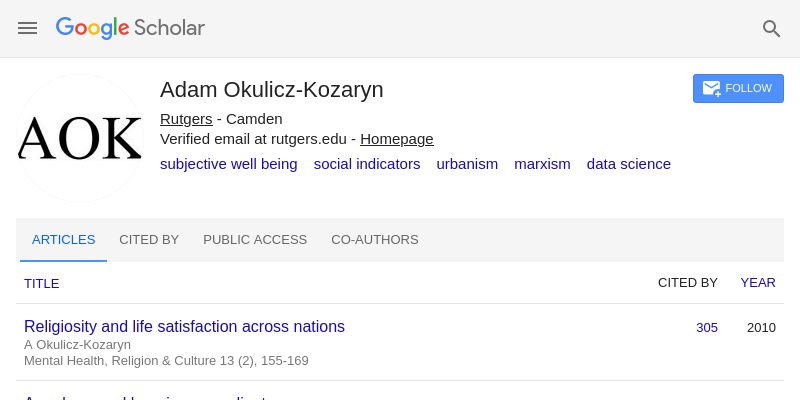
\includegraphics[height=2in]{a.png}
  \caption{\label{a}Note we stick to \texttt{lifesat} tag (life satisfaction) as in the
    original dataset, but again it is rather momentary affective happiness than
    global cognitive evaluation of one's life as a whole, life satisfaction
    term used in SWB literature.}
\end{figure}
%old way couldnt get size
% \begin{figure}[H]
% %!!!first time need to run pdflatex --shell-escape hfgi.tex
% \includegraphicsfromurl{https://raw.githubusercontent.com/theaok/hfgi/refs/heads/main/a.png}{a.png}
% \caption{\label{a}}
% \end{figure}

 
 One nuance is that \texttt{posfunct} and \texttt{vitality} columns show the
 lowest levels (dark red) not in the very largest counties in the last row
 ``204.9k-10077.3k,'' but in slightly smaller but still above the median
 population size rows. 


Also note quite large substantive differences.
Energy/vitality index \texttt{eneI} has a  12\% (.35/.31) difference between 1st and
10th deciles. \texttt{Posfunct} and \texttt{vitality} are even bigger
percentage differences.

 

Table \ref{b} repeats the exercise but for happiness index  \texttt{swbI} and individual
 measures. Here as expected and shown in the literature \citep{aok11a} in second
 colored column \texttt{lifesat}, life satisfaction raises from its lowest level
 for largest counties in last decile of population to its highest level for the
 smallest counties in first decile of population. But this pattern is only
 observed for this one column. Overall, in all other columns the pattern tends to
 be of lowest wellbeing in 10th decile as expected, but also in the 1st
 decile. Still, the urban-rural happiness gradient hypothesis \citep{aok11a}
 holds as the counties with highest wellbeing scores are the smallest counties
 in 2nd, 3rd, and 4th population size deciles (5.1k-18.5k), and some of the
 lowest wellbeing scores are also in the second highest 9th population
 decile. Overall, we find lowest happiness in 1st and 10th population deciles
 and highest in 2nd-4th population deciles. While as expected smaller 2nd-4th
 deciles counties tends to be happier and largest 9th-10th deciles counties tend
 to be less happy, it is also the very smallest counties in 1st deciles that are
 unhappy.

% %!!!first time need to run pdflatex --shell-escape hfgi.tex
\downloadimage{https://raw.githubusercontent.com/theaok/hfgi/refs/heads/main/b.png}{b.png}
\begin{figure}[htbp]
  \centering
  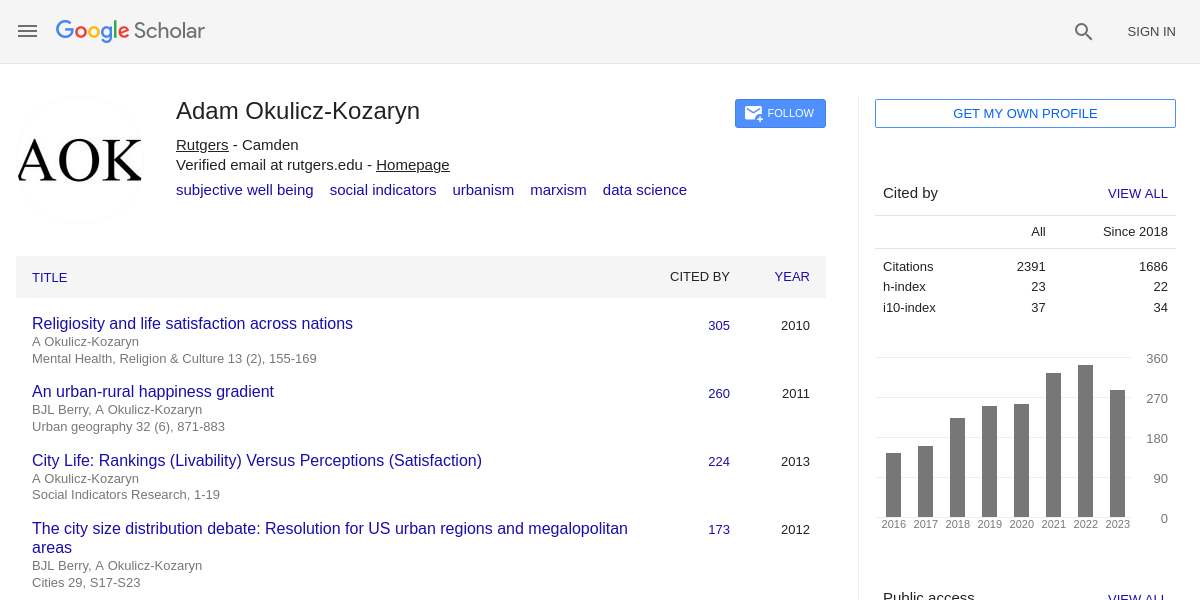
\includegraphics[height=2in]{b.png}
  \caption{\label{b}This figure was pulled directly from a web URL.}
\end{figure}


 \texttt{Lifesat} is as expected in the literature, and do note huge urban-rural
 happiness gradient change all the way from .06 for 10th decile to .15 for the
 1st decile, $>$2x difference. 
 %
 But \texttt{happiness} is almost the other way round from lowest in smaller
 counties to larger in larger counties (but not very largest), slightly an 
  inverted U-shape with maximum at 6th decile (25.6k-36.7k) and
  \texttt{optimism} is very similar. \texttt{Hope} has a clear inverted U-shape
  with maximum at 6th decile and minimums at 1st and 10th deciles.  
 %
 Still, overall from the happiness index
 \texttt{swbI} (and \texttt{innerpeace}) it is not the very smallest ones like $<$5.1k, but also small ones already at $<$18.5k.
 
 There are also some nuances, for instance 6th decile (25.6k-36.7k)
 scores highest on \texttt{happiness}, \texttt{optimism}, and
 \texttt{hope}.\footnote{Along with 3rd decile.} Hence, for these measures there
 is evidence of inverted U-shape: highest happiness is around median population
 size and lowest in smallest and largest counties.  




\subsection{Across counties}

We turn to mapping\footnote{Here as maps show, it is only contiguous US, but in other analyses there were
  few additional observations from Alaska and Hawaii.} energy/vitality index
\texttt{eneI} and happiness index \texttt{swbI} across counties. \texttt{EneI} is in figure \ref{eneI}.


% %!!!first time need to run pdflatex --shell-escape hfgi.tex
\downloadimage{https://raw.githubusercontent.com/theaok/hfgi/refs/heads/main/eneI.pdf}{eneI.pdf}
\begin{figure}[h!]
  \centering
  \includegraphics[height=4.5in]{eneI.pdf}
  \caption{\label{eneI} Energy/vitality index.}
\end{figure}

South does not surprise. As expected, the energy/vitality is low in South:
especially in  Mississippi and Louisiana, but also in most parts of Texas and
Alabama. Second comes Midwest, no surprise there either. Ohio is the lowest
almost all low energy/vitality, and then most of Pennsylvania and and about half
of West Virginia and Michigan (South Michigan is low, North Michigan is high). 

Also about half of  Oklahoma and Kansas are low on energy/vitality. On West coast, perhaps
 surprisingly about half or Oregon is low on energy/vitality.
 And in Georgia and Arkansas about third.

As opposed to dull South and Midwest, there is definitely more energy/vitality
in North East, for instance in New Jersey--one would think. But our results
disagree--there is not much difference, if any. Dull and low energy South does contrast
with upbeat and high energy North East--it is just that the energy may not be
that good after all--stressed and neurotic. This concludes our general
list of low energy/vitality states, but do note many red spots throughout the US
and in other states. In appendix we have a top and bottom 100 ranking tables
with all variables. Also in appendix are more detailed maps with more color bins. Overall
they are very similar, so we stick with simplified exposition presented here. The extremes remain the same: dark red and dark green
but there is much more gradation for mid-levels from light green through yellow
to light red.


Turning now to high energy/vitality: in general West and North but not coastal/Pacific West: not Oregon, neither
California. Colorado seems the highest energy/vitality, but also Utah, Wyoming, Montana, and Idaho.

% and many interesting negative spatial corr outliers
% (later lisa clustering)



The happiness map in figure \ref{swbI} broadly agrees with energy/vitality map
in figure \ref{eneI}, and the correlation between the two is .83, for a
scatterplot see appendix. There are few differences, however, for instance, Tennessee,
Arkansas, and Missouri have more happiness than energy/vitality, North East,
too, except New Jersey that is equally unhappy as it has low energy/vitality.  
As opposed to above energy/vitality index in the above map \ref{eneI}, the below
happiness map in figure \ref{swbI} is not entirely new. 

% %!!!first time need to run pdflatex --shell-escape hfgi.tex
\downloadimage{https://raw.githubusercontent.com/theaok/hfgi/refs/heads/main/swbI.pdf}{swbI.pdf}
\begin{figure}[h!]
  \centering
  \includegraphics[height=4.5in]{swbI.pdf}
  \caption{\label{swbI}This figure was pulled directly from a web URL.}
\end{figure}

Results in figure \ref{swbI} broadly agree at state level with % ``Figure
% 1. Average word happiness for geotagged tweets in all US states collected during
% calendar year 2011'' in
 \citet{mitchell13}.
Much of the results in our figure \ref{swbI} also seem to agree at county level with % ``Figure
% 5. Map showing happiness of all tweets collected from the lower 48 US states
% during 2011'' in
 \citet{mitchell13}, but it is difficult to say as
map averages at county level, while \citet{mitchell13} map closer to actual tweet locations and there are multiple points per county and it is difficult to estimate the average.\footnote{Note that there is also an an Atlantic article that covers the arxiv version of their study.https://www.theatlantic.com/technology/archive/2013/02/the-geography-of-happiness-according-to-10-million-tweets/273286/}


\citet{kjell2023towards} shows a map similar to our county estimates
in figure 5.1C citing \citet{jaidka2020estimating}.
It looks like their sample of 1.5b is close to ours. But the results are
different possibly due to their ``interpolation of missing counties provided through a Gaussian process model using demographic and socioeconomic similarity between counties''
\citep[][fig. 5.1C caption]{kjell2023towards}: 
Alabama, Louisiana, and Mississippi are not unhappy, neither is North East, but
Midwest is least happy (we find it unhappy but not as unhappy as Alabama,
Louisiana, and Mississippi).

But maybe the most striking difference is that urban
counties marked in their figure 5.1C with city names all appear to be the
very happiest counties of all (dark green). Except Los Angeles and Miami (2nd shade of
green, still very happy), Phoenix (yellow; average happiness), and per New York
and New Orleans we cannot really tell as the black city dots cover
polygons. Curiously, World Happiness Report and Gallup argue urban happiness
despite data showing the contrary--see discussion
in \citet{aok21}. For instance see
  \url{https://news.gallup.com/opinion/gallup/315857/degree-urbanisation-effect-happiness.aspx}.   


\subsection{Zooming in on the largest cities}

Table \ref{c} shows wellbeing metrics for 20 largest counties. It is important
to keep in mind that all data including population pertains to a 
county, not city, for instance Santa Ana is only about 300k but Orange county is
about 3m. But we are using cities for ease of interpretations.
First, summarizing all indicators as happy or unhappy
as for most counties there is a clear pattern. First 4 numeric columns are
energy/vitality (\texttt{eneI}, \texttt{posfunct}, \texttt{vitality}, \texttt{energy})	
 and subsequent 6 numeric columns are happiness (\texttt{swbI},
 \texttt{lifesat}, \texttt{happiness}, \texttt{innerpeace},
 \texttt{optimism},\texttt{purpose}, and \texttt{hope}).
 
Happy counties are sunny places, but outside of unhappy Texas, and many coastal
like Los Angeles, Phoenix, San Diego, Santa Ana, Miami, Las Vegas, San Jose and
Ft Lauderdale. Also happy are cold but coastal Seattle and Manhattan (New York
County).


Detroit and Houston are the least happy. In addition to Houston, there are 2
other unhappy Texas cities, Dallas and Forth Worth. NYC Queens and Brooklyn are
not too happy either in sharp contrast to very happy Manhattan.


Then few interesting nuances. For instance 3 Texas cities Dallas, Forth Worth
(neighbors), and San Antonio score poorly on energy/vitality (first 4 numeric
columns) but quite well on happiness (subsequent 6 numeric columns).


At the bottom of the table is comparison to deciles from earlier figures (note that comparison
colors in the table differ as they are scaled to current table). Decile 1 tends
to be higher than mean of deciles 2-4. Of the largest metropolises some score
better or worse than decile averages. 

Highest and lowest both energy/vitality and happiness
    tends to be in small counties, below median population size (see appendix).
In appendix we also provide a full list of top and bottom counties on
energy/vitality index \texttt{eneI}. 

% %!!!first time need to run pdflatex --shell-escape hfgi.tex
\downloadimage{https://raw.githubusercontent.com/theaok/hfgi/refs/heads/main/c.png}{c.png}
\begin{figure}[htbp]
  \centering
  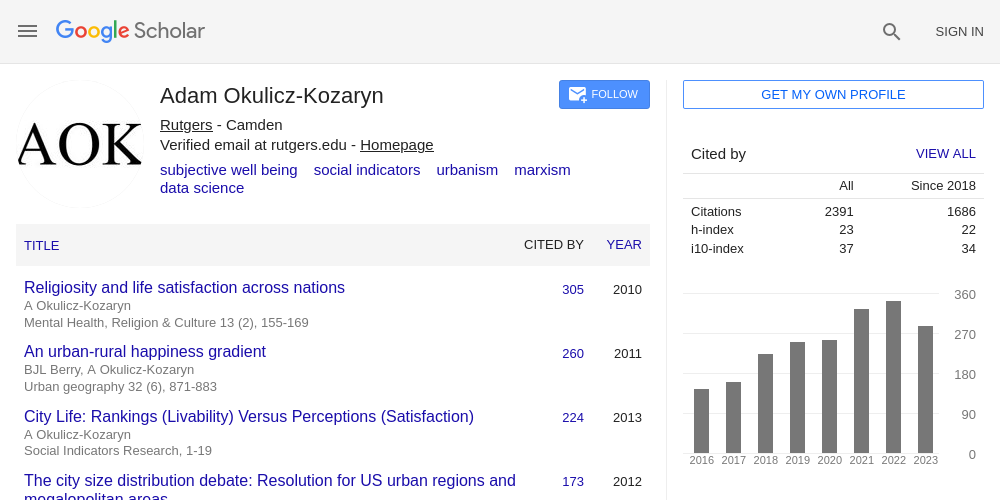
\includegraphics[height=4.5in]{c.png}
  \caption{\label{c}Energy/vitality and happiness for 20 largest
    counties. Counties are sorted on population. At the bottom for comparison
    averages for 1st decile, 2-3rd deciles, and 10th decile. }
\end{figure}


Again, \citet{kjell2023towards} has a map (fig 5.1C) similar to our county
estimates, and the results differ. Their map has several large cities marked on
it--and they appear to be the very happiest counties of all (most seem to be dark green).
 While the black dot marking the city covers most or all of the city-counties,
 the metropolitan area bordering counties that are clearly visible are very
 happy, which already is surprising. Except Los Angeles and Miami (2nd shade of
green, still very happy), and Phoenix (yellow; average happiness), and unclear New York
and New Orleans (small counties completely covered by the black dot), it seems
that all these large cities are very happy. They are from West to East: Seattle,
Los Angeles, Salt Lake City, Phoenix, Denver, Minneapolis, Chicago, Houston,
Atlanta, Washington, and Miami. For instance we have found Houston in  table
\ref{c} to be unhappy, likewise earlier in county maps all of Houston vicinity
wasn't happy. 





\section{Conclusion and discussion}

This is the first study of geography of energy/vitality, where we
find a very clear urban-rural gradient with energy/vitality raising from its
lowest levels for large counties to highest level in small
counties. Energy/vitality may be actually more important than happiness and at
least as important, and it is striking that we know nothing about its geography.  


%TODO !!!! have input here aok_var_des



% %table centered on decimal points:)
% \begin{table}[H]\centering\footnotesize
% \caption{\label{freq_im_god} importance of God}
% \begin{tabular} {@{} lrrrr @{}}   \hline 
% Item& Number & Per cent   \\ \hline
% 1(not at all)&    9,285&  9\\
% 2&    3,555&        3\\
% 3&    3,937&        4\\
% 4&    2,888&        3\\
% 5&    7,519&        7\\
% 6&    5,175&        5\\
% 7&    6,050&        6\\
% 8&    8,067&        8\\
% 9&    8,463&        8\\
% 10&   52,385&       49\\
% Total&  107,324&      100\\ \hline
% \end{tabular}\end{table}


% % Define block styles
% \tikzstyle{block} = [rectangle, draw, fill=black!20, 
%     text width=10em, text centered, rounded corners, minimum height=4em]
% \tikzstyle{b} = [rectangle, draw,  
%     text width=6em, text centered, rounded corners, minimum height=4em]
% \tikzstyle{line} = [draw, -latex']
% \tikzstyle{cloud} = [draw, ellipse,fill=black!20, node distance = 5cm,
%     minimum height=2em]
    
% \begin{tikzpicture}[node distance = 2cm, auto]
%     % Place nodes
%     \node [block] (lib) {liberalism, egalitarianism, welfare};
%     \node [block, below of=lib] (con) {conservatism, competition, individualism};
%     \node [cloud, right of=con] (ls) {well-being};
%     \node [block, below of=ls] (cul) {genes, culture};
%     \node [b, left of =lib, node distance = 4cm] (c) {country-level};
%     \node [b, left of =con,  node distance = 4cm] (c) {person-level};
%     % Draw edges
%     \path [line] (lib) -- (ls);
%     \path [line] (con) -- (ls);
%     \path [line,dashed] (cul) -- (ls);
% \end{tikzpicture}


%PUT THIS NOTE, polish and put to /root/author_what_data --ALWAYS
%stick here stuff as i run it!!! maybe comment out later...


%TODO: have separate som-r.tex as opposed to having it below; and in paper say
%see online appendix!

\newpage
\bibliography{/home/aok/papers/root/tex/ebib.bib,hfgi.bib}

\newpage

 \section*{\Huge ONLINE APPENDIX}
 \textbf{[note: this section will NOT be a part of the final version of
   the manuscript, but will be available online instead]} %hence everything below
%                                 %is organized byu section, not subsection
% !!!
% have most of the stuff outputted to online appendix:)--start with that and then
% select stuff to paper--have brief narrative describng patterns in online app too
% !!!

\subsection{Additional results}

% %!!!first time need to run pdflatex --shell-escape hfgi.tex
\downloadimage{https://raw.githubusercontent.com/theaok/hfgi/refs/heads/main/eneIf.pdf}{eneIf.pdf}
\begin{figure}[htbp]
  \centering
  \includegraphics[height=4.5in]{eneIf.pdf}
  \caption{more classes This figure was pulled directly from a web URL.}
\end{figure}

% %!!!first time need to run pdflatex --shell-escape hfgi.tex
\downloadimage{https://raw.githubusercontent.com/theaok/hfgi/refs/heads/main/swbIf.pdf}{swbIf.pdf}
\begin{figure}[htbp]
  \centering
  \includegraphics[height=4.5in]{swbIf.pdf}
  \caption{more classes This figure was pulled directly from a web URL.}
\end{figure}

\downloadimage{https://raw.githubusercontent.com/theaok/hfgi/refs/heads/main/eneIswbISc.png}{eneIswbISc.png}              
\begin{figure}[htbp]
  \centering
  \includegraphics[height=2.5in]{eneIswbISc.png}
  \caption{\label{eneIswbISc} Correlation is 0.83.}
\end{figure}

\downloadimage{https://raw.githubusercontent.com/theaok/hfgi/refs/heads/main/topBotA.png}{topBotA.png}              
\begin{figure}[htbp]
  \centering
  \includegraphics[height=3.5in]{topBotA.png}
  \caption{\label{topBotA} Highest and lowest bot energy/vitality and happiness
    tends to be in small counties, below median population size.}
\end{figure}



\begin{table}
  \centering
{\renewcommand{\arraystretch}{.5}\tiny
  \begin{tabular}{llrrrrrrrrrrrr} \hline STNAME & CTYNAME & POPESTIMATE2015 &
    eneI & posfunct & vitality & energy & swbI & lifesat & happiness &
    innerpeace & optimism & purpose & hope \\ \hline Montana & Golden Valley
    County & 818 & 0.65 & 0.64 & 0.70 & 0.60 & 0.19 &
    -0.02 & 0.19 & -0.11 & 0.11 & 0.50 & 0.47 \\
    Colorado & Jackson County & 1352 & 0.64 & 0.61 & 0.68 & 0.64
    & 0.49 & 0.43 & 0.48 & 0.39 & 0.41 & 0.64 & 0.59
    \\ Colorado & Hinsdale County & 762 & 0.61 & 0.62 & 0.65 &
    0.56 & 0.48 & 0.40 & 0.50 & 0.40 & 0.44 & 0.54 &
    0.61 \\ Montana & Musselshell County & 4631 & 0.59 & 0.59 &
    0.57 & 0.61 & 0.39 & 0.24 & 0.39 & 0.28 & 0.33 &
    0.56 & 0.52 \\ Wyoming & Sublette County & 10064 & 0.59 &
    0.57 & 0.61 & 0.58 & 0.38 & 0.19 & 0.33 & 0.31 &
    0.27 & 0.64 & 0.56 \\ Alaska & Skagway Municipality & 1090 &
    0.58 & 0.57 & 0.62 & 0.55 & 0.45 & 0.40 & 0.41 &
    0.33 & 0.34 & 0.59 & 0.60 \\ Wyoming & Teton County & 23083
    & 0.58 & 0.55 & 0.60 & 0.59 & 0.47 & 0.38 & 0.43
    & 0.32 & 0.40 & 0.64 & 0.62 \\ California & Alpine County &
    1080 & 0.58 & 0.57 & 0.61 & 0.55 & 0.43 & 0.34 &
    0.40 & 0.33 & 0.30 & 0.58 & 0.61 \\ Utah & Rich County &
    2301 & 0.58 & 0.57 & 0.59 & 0.56 & 0.47 & 0.42 &
    0.49 & 0.35 & 0.44 & 0.56 & 0.55 \\ Colorado & Saguache
    County & 6250 & 0.56 & 0.57 & 0.53 & 0.59 & 0.45 &
    0.35 & 0.45 & 0.38 & 0.40 & 0.53 & 0.58 \\ Colorado
    & Ouray County & 4611 & 0.56 & 0.53 & 0.56 & 0.59 & 0.46
    & 0.38 & 0.46 & 0.33 & 0.41 & 0.56 & 0.62 \\
    Colorado & Dolores County & 1980 & 0.55 & 0.59 & 0.57 & 0.50
    & 0.41 & 0.38 & 0.42 & 0.27 & 0.34 & 0.53 & 0.50
    \\ Colorado & San Juan County & 690 & 0.55 & 0.57 & 0.57 &
    0.53 & 0.45 & 0.41 & 0.49 & 0.30 & 0.38 & 0.54 &
    0.59 \\ Utah & Garfield County & 4966 & 0.55 & 0.56 & 0.57 &
    0.53 & 0.40 & 0.28 & 0.41 & 0.35 & 0.32 & 0.58 &
    0.48 \\ Minnesota & Cook County & 5249 & 0.55 & 0.51 & 0.57
    & 0.57 & 0.44 & 0.36 & 0.44 & 0.35 & 0.35 & 0.54
    & 0.56 \\ Montana & Madison County & 8033 & 0.55 & 0.55 &
    0.54 & 0.57 & 0.40 & 0.35 & 0.38 & 0.31 & 0.26 &
    0.54 & 0.57 \\ Washington & San Juan County & 16155 & 0.55 &
    0.53 & 0.54 & 0.58 & 0.41 & 0.30 & 0.43 & 0.32 &
    0.36 & 0.50 & 0.53 \\ Montana & Treasure County & 680 & 0.55
    & 0.57 & 0.53 & 0.54 & 0.30 & 0.24 & 0.31 & 0.17
    & 0.25 & 0.34 & 0.48 \\ Tennessee & Hancock County & 6577 &
    0.54 & 0.51 & 0.53 & 0.59 & 0.36 & 0.24 & 0.40 &
    0.19 & 0.37 & 0.44 & 0.52 \\ Colorado & Mineral County & 742
    & 0.54 & 0.55 & 0.58 & 0.50 & 0.42 & 0.38 & 0.40
    & 0.29 & 0.35 & 0.53 & 0.54 \\ Colorado & Grand County &
    14742 & 0.54 & 0.51 & 0.56 & 0.56 & 0.41 & 0.28 &
    0.42 & 0.25 & 0.36 & 0.55 & 0.58 \\ Tennessee & Perry
    County & 7855 & 0.54 & 0.61 & 0.52 & 0.49 & 0.40 &
    0.35 & 0.34 & 0.29 & 0.32 & 0.62 & 0.46 \\ Hawaii &
    Kauai County & 71052 & 0.54 & 0.51 & 0.56 & 0.54 & 0.43
    & 0.32 & 0.45 & 0.32 & 0.38 & 0.52 & 0.57 \\ Hawaii
    & Maui County & 163993 & 0.53 & 0.51 & 0.55 & 0.54 &
    0.43 & 0.31 & 0.45 & 0.31 & 0.38 & 0.57 & 0.56
    \\ Utah & Daggett County & 1107 & 0.53 & 0.50 & 0.59 & 0.51
    & 0.38 & 0.34 & 0.37 & 0.35 & 0.35 & 0.39 & 0.47
    \\ Wyoming & Lincoln County & 18788 & 0.53 & 0.52 & 0.52 &
    0.55 & 0.37 & 0.25 & 0.33 & 0.23 & 0.25 & 0.58 &
    0.60 \\ Idaho & Boise County & 6963 & 0.53 & 0.51 & 0.53 &
    0.53 & 0.39 & 0.27 & 0.40 & 0.27 & 0.32 & 0.52 &
    0.53 \\ Colorado & Custer County & 4434 & 0.53 & 0.53 & 0.49
    & 0.56 & 0.43 & 0.34 & 0.44 & 0.35 & 0.36 & 0.51
    & 0.58 \\ Montana & Powder River County & 1768 & 0.52 & 0.53 &
    0.55 & 0.49 & 0.29 & 0.16 & 0.26 & 0.12 & 0.18 &
    0.50 & 0.54 \\ Colorado & San Miguel County & 7850 & 0.52 &
    0.51 & 0.52 & 0.54 & 0.43 & 0.35 & 0.46 & 0.27 &
    0.38 & 0.57 & 0.57 \\ Utah & Kane County & 7045 & 0.52 &
    0.51 & 0.53 & 0.53 & 0.41 & 0.32 & 0.40 & 0.32 &
    0.33 & 0.53 & 0.54 \\ California & Mariposa County & 17653 &
    0.52 & 0.51 & 0.54 & 0.51 & 0.39 & 0.35 & 0.41 &
    0.30 & 0.34 & 0.50 & 0.47 \\ Utah & Grand County & 9530 &
    0.52 & 0.52 & 0.53 & 0.51 & 0.43 & 0.35 & 0.42 &
    0.31 & 0.37 & 0.55 & 0.55 \\ Montana & Stillwater County &
    9419 & 0.52 & 0.51 & 0.47 & 0.58 & 0.34 & 0.21 &
    0.35 & 0.20 & 0.24 & 0.48 & 0.54 \\ Minnesota &
    Clearwater County & 8794 & 0.52 & 0.53 & 0.46 & 0.57 &
    0.39 & 0.28 & 0.39 & 0.31 & 0.36 & 0.50 & 0.51
    \\ Wisconsin & Price County & 13577 & 0.52 & 0.50 & 0.50 &
    0.56 & 0.38 & 0.25 & 0.38 & 0.30 & 0.35 & 0.47 &
    0.56 \\ Colorado & Costilla County & 3576 & 0.52 & 0.50 &
    0.49 & 0.57 & 0.43 & 0.34 & 0.44 & 0.33 & 0.39 &
    0.49 & 0.56 \\ Alaska & Haines Borough & 2519 & 0.52 & 0.50
    & 0.57 & 0.48 & 0.36 & 0.33 & 0.31 & 0.28 & 0.16
    & 0.55 & 0.51 \\ Minnesota & Lake County & 10540 & 0.52 &
    0.51 & 0.51 & 0.54 & 0.40 & 0.37 & 0.39 & 0.26 &
    0.33 & 0.53 & 0.53 \\ Colorado & Lake County & 7455 & 0.52 &
    0.49 & 0.53 & 0.54 & 0.42 & 0.29 & 0.42 & 0.30 &
    0.36 & 0.57 & 0.56 \\ Colorado & Pitkin County & 17962 &
    0.52 & 0.49 & 0.49 & 0.57 & 0.42 & 0.32 & 0.46 &
    0.28 & 0.38 & 0.50 & 0.58 \\ Montana & Petroleum County &
    475 & 0.52 & 0.56 & 0.45 & 0.53 & 0.37 & 0.19 &
    0.36 & 0.39 & 0.20 & 0.54 & 0.53 \\ Colorado & Crowley
    County & 5633 & 0.51 & 0.50 & 0.46 & 0.58 & 0.36 &
    0.30 & 0.33 & 0.25 & 0.23 & 0.65 & 0.40 \\ North
    Dakota & Billings County & 950 & 0.51 & 0.50 & 0.50 & 0.54 &
    0.42 & 0.34 & 0.38 & 0.32 & 0.34 & 0.58 & 0.58
    \\ North Carolina & Swain County & 14325 & 0.51 & 0.51 & 0.52 &
    0.50 & 0.42 & 0.29 & 0.42 & 0.33 & 0.36 & 0.57 &
    0.57 \\ New Mexico & Catron County & 3480 & 0.51 & 0.48 &
    0.50 & 0.55 & 0.40 & 0.40 & 0.39 & 0.26 & 0.31 &
    0.52 & 0.54 \\ Nebraska & Boyd County & 2004 & 0.51 & 0.55 &
    0.46 & 0.52 & 0.43 & 0.35 & 0.43 & 0.34 & 0.36 &
    0.57 & 0.55 \\ Idaho & Adams County & 3891 & 0.51 & 0.49 &
    0.51 & 0.52 & 0.37 & 0.25 & 0.39 & 0.20 & 0.31 &
    0.47 & 0.57 \\ Colorado & Baca County & 3554 & 0.51 & 0.48 &
    0.54 & 0.50 & 0.35 & 0.28 & 0.28 & 0.29 & 0.18 &
    0.54 & 0.51 \\ Nebraska & Garfield County & 2013 & 0.50 &
    0.49 & 0.50 & 0.53 & 0.38 & 0.27 & 0.32 & 0.32 &
    0.30 & 0.53 & 0.55 \\ Virginia & Rappahannock County & 7409 &
    0.50 & 0.51 & 0.44 & 0.56 & 0.40 & 0.27 & 0.45 &
    0.28 & 0.36 & 0.51 & 0.54 \\ New York & Hamilton County &
    4700 & 0.50 & 0.45 & 0.50 & 0.56 & 0.36 & 0.18 &
    0.39 & 0.26 & 0.29 & 0.54 & 0.47 \\ Hawaii & Hawaii
    County & 196111 & 0.50 & 0.49 & 0.52 & 0.50 & 0.37 &
    0.30 & 0.36 & 0.29 & 0.21 & 0.51 & 0.52 \\ Montana &
    Flathead County & 95940 & 0.50 & 0.50 & 0.45 & 0.55 &
    0.41 & 0.27 & 0.42 & 0.27 & 0.37 & 0.56 & 0.55
    \\ Montana & Meagher County & 1822 & 0.50 & 0.52 & 0.46 &
    0.51 & 0.31 & 0.22 & 0.33 & 0.18 & 0.22 & 0.41 &
    0.49 \\ Nevada & Storey County & 3881 & 0.50 & 0.48 & 0.43 &
    0.58 & 0.40 & 0.27 & 0.42 & 0.26 & 0.36 & 0.55 &
    0.56 \\ Washington & Skamania County & 11386 & 0.50 & 0.50 &
    0.48 & 0.50 & 0.38 & 0.29 & 0.40 & 0.29 & 0.29 &
    0.50 & 0.51 \\ South Dakota & Jackson County & 3281 & 0.49 &
    0.50 & 0.48 & 0.50 & 0.37 & 0.30 & 0.39 & 0.25 &
    0.30 & 0.49 & 0.51 \\ Colorado & Summit County & 30064 &
    0.49 & 0.46 & 0.49 & 0.53 & 0.39 & 0.27 & 0.43 &
    0.25 & 0.35 & 0.51 & 0.53 \\ South Dakota & Custer County &
    8456 & 0.49 & 0.47 & 0.48 & 0.53 & 0.39 & 0.35 &
    0.38 & 0.27 & 0.30 & 0.52 & 0.51 \\ Idaho & Idaho County
    & 16312 & 0.49 & 0.50 & 0.45 & 0.53 & 0.39 & 0.29 &
    0.39 & 0.28 & 0.31 & 0.53 & 0.54 \\ California & Sierra
    County & 2990 & 0.49 & 0.51 & 0.49 & 0.48 & 0.32 &
    0.32 & 0.24 & 0.31 & 0.06 & 0.48 & 0.52 \\ Colorado
    & Clear Creek County & 9246 & 0.49 & 0.51 & 0.55 & 0.41 &
    0.37 & 0.35 & 0.35 & 0.14 & 0.27 & 0.58 & 0.56
    \\ Oregon & Wallowa County & 6810 & 0.49 & 0.56 & 0.55 &
    0.36 & 0.37 & 0.30 & 0.33 & 0.31 & 0.25 & 0.57 &
    0.42 \\ Utah & Wayne County & 2689 & 0.49 & 0.49 & 0.48 &
    0.49 & 0.41 & 0.35 & 0.41 & 0.32 & 0.32 & 0.49 &
    0.55 \\ Vermont & Lamoille County & 25265 & 0.49 & 0.48 &
    0.46 & 0.53 & 0.40 & 0.26 & 0.42 & 0.27 & 0.35 &
    0.55 & 0.56 \\ Nevada & Pershing County & 6620 & 0.49 & 0.48
    & 0.43 & 0.56 & 0.31 & 0.14 & 0.34 & 0.14 & 0.22
    & 0.52 & 0.50 \\ Montana & Carbon County & 10404 & 0.49 &
    0.46 & 0.48 & 0.52 & 0.35 & 0.23 & 0.35 & 0.17 &
    0.23 & 0.54 & 0.58 \\ Oregon & Hood River County & 22925 &
    0.49 & 0.51 & 0.50 & 0.45 & 0.35 & 0.21 & 0.39 &
    0.25 & 0.29 & 0.46 & 0.51 \\ Oregon & Wheeler County & 1327
    & 0.48 & 0.57 & 0.52 & 0.36 & 0.37 & 0.32 & 0.37
    & 0.30 & 0.23 & 0.53 & 0.46 \\ Montana & Granite County &
    3160 & 0.48 & 0.51 & 0.46 & 0.49 & 0.37 & 0.29 &
    0.36 & 0.24 & 0.31 & 0.54 & 0.51 \\ Montana & Jefferson
    County & 11576 & 0.48 & 0.47 & 0.45 & 0.53 & 0.33 &
    0.23 & 0.33 & 0.24 & 0.23 & 0.44 & 0.49 \\ Colorado
    & Eagle County & 53863 & 0.48 & 0.46 & 0.45 & 0.55 &
    0.40 & 0.28 & 0.44 & 0.25 & 0.37 & 0.49 & 0.56
    \\ Colorado & Montezuma County & 25763 & 0.48 & 0.49 & 0.43 &
    0.53 & 0.37 & 0.24 & 0.38 & 0.25 & 0.34 & 0.48 &
    0.51 \\ Idaho & Fremont County & 12824 & 0.48 & 0.48 & 0.44
    & 0.53 & 0.34 & 0.23 & 0.36 & 0.22 & 0.27 & 0.47
    & 0.51 \\ Missouri & Hickory County & 9269 & 0.48 & 0.49 &
    0.45 & 0.50 & 0.40 & 0.28 & 0.42 & 0.31 & 0.33 &
    0.52 & 0.52 \\ Kansas & Morris County & 5630 & 0.48 & 0.48 &
    0.38 & 0.57 & 0.41 & 0.32 & 0.35 & 0.33 & 0.34 &
    0.55 & 0.58 \\ Michigan & Keweenaw County & 2124 & 0.48 &
    0.48 & 0.45 & 0.50 & 0.33 & 0.28 & 0.34 & 0.22 &
    0.25 & 0.42 & 0.49 \\ South Dakota & Marshall County & 4830 &
    0.48 & 0.52 & 0.39 & 0.53 & 0.39 & 0.30 & 0.35 &
    0.25 & 0.30 & 0.54 & 0.57 \\ Colorado & Chaffee County &
    18635 & 0.48 & 0.49 & 0.44 & 0.50 & 0.38 & 0.24 &
    0.40 & 0.25 & 0.35 & 0.50 & 0.54 \\ Wisconsin & Buffalo
    County & 13245 & 0.48 & 0.46 & 0.44 & 0.54 & 0.38 &
    0.32 & 0.34 & 0.31 & 0.26 & 0.51 & 0.54 \\ South
    Dakota & Gregory County & 4195 & 0.48 & 0.49 & 0.46 & 0.48 &
    0.31 & 0.29 & 0.26 & 0.28 & 0.16 & 0.44 & 0.47
    \\ Montana & Sweet Grass County & 3618 & 0.48 & 0.46 & 0.43 &
    0.54 & 0.32 & 0.30 & 0.30 & 0.14 & 0.22 & 0.45 &
    0.49 \\ Montana & Lake County & 29482 & 0.47 & 0.48 & 0.38 &
    0.57 & 0.42 & 0.22 & 0.47 & 0.25 & 0.42 & 0.58 &
    0.59 \\ Colorado & Conejos County & 8064 & 0.47 & 0.51 &
    0.45 & 0.46 & 0.38 & 0.31 & 0.41 & 0.30 & 0.30 &
    0.45 & 0.52 \\ Tennessee & Van Buren County & 5697 & 0.47 &
    0.49 & 0.47 & 0.46 & 0.38 & 0.24 & 0.38 & 0.29 &
    0.32 & 0.53 & 0.52 \\ Indiana & Brown County & 15003 & 0.47
    & 0.43 & 0.46 & 0.52 & 0.38 & 0.28 & 0.40 & 0.20
    & 0.34 & 0.52 & 0.52 \\ Colorado & Sedgwick County & 2373 &
    0.47 & 0.46 & 0.45 & 0.51 & 0.31 & 0.19 & 0.34 &
    0.21 & 0.22 & 0.43 & 0.47 \\ Montana & Toole County & 5083 &
    0.47 & 0.46 & 0.36 & 0.59 & 0.38 & 0.21 & 0.41 &
    0.20 & 0.37 & 0.52 & 0.54 \\ North Dakota & Oliver County &
    1866 & 0.47 & 0.47 & 0.47 & 0.48 & 0.32 & 0.07 &
    0.40 & 0.10 & 0.36 & 0.39 & 0.59 \\ Tennessee & Fentress
    County & 17974 & 0.47 & 0.49 & 0.38 & 0.53 & 0.40 &
    0.30 & 0.30 & 0.29 & 0.37 & 0.58 & 0.58 \\ South
    Dakota & Brule County & 5239 & 0.47 & 0.46 & 0.44 & 0.50 &
    0.32 & 0.18 & 0.32 & 0.20 & 0.24 & 0.48 & 0.49
    \\ Hawaii & Honolulu County & 991755 & 0.47 & 0.44 & 0.46 &
    0.50 & 0.36 & 0.23 & 0.40 & 0.25 & 0.32 & 0.47 &
    0.51 \\ North Carolina & Avery County & 17494 & 0.47 & 0.45 &
    0.47 & 0.49 & 0.38 & 0.29 & 0.39 & 0.25 & 0.33 &
    0.49 & 0.55 \\ Wyoming & Niobrara County & 2504 & 0.47 &
    0.45 & 0.49 & 0.47 & 0.29 & 0.21 & 0.24 & 0.17 &
    0.17 & 0.43 & 0.52 \\ Alaska & Ketchikan Gateway Borough & 13737
    & 0.47 & 0.45 & 0.45 & 0.50 & 0.37 & 0.24 & 0.37
    & 0.25 & 0.29 & 0.53 & 0.53 \\ Maine & Hancock County &
    54280 & 0.47 & 0.44 & 0.45 & 0.51 & 0.37 & 0.28 &
    0.39 & 0.24 & 0.34 & 0.45 & 0.53 \\ Montana & Judith
    Basin County & 1932 & 0.47 & 0.47 & 0.38 & 0.55 & 0.39 &
    0.23 & 0.39 & 0.31 & 0.35 & 0.48 & 0.58 \\ Montana &
    Fallon County & 3172 & 0.47 & 0.45 & 0.40 & 0.54 & 0.28
    & 0.28 & 0.16 & 0.17 & 0.15 & 0.46 & 0.47 \\ Alaska
    & Bristol Bay Borough & 906 & 0.47 & 0.44 & 0.50 & 0.46 &
    0.31 & 0.18 & 0.32 & 0.20 & 0.22 & 0.46 & 0.48
    \\ \hline \end{tabular}
}
  \caption{Top 100 Sorted on \texttt{eneI}.}
\end{table}

 
\begin{table}
  \centering
{\renewcommand{\arraystretch}{.5}\tiny
  \begin{tabular}{llrrrrrrrrrrrr}
\hline
STNAME & CTYNAME & POPESTIMATE2015 & eneI & posfunct & vitality & energy & swbI & lifesat & happiness & innerpeace & optimism & purpose & hope \\
\hline
Texas & Jasper County & 35268 & 0.22 & 0.20 & 0.12 & 0.34 & 0.18 & 0.03 & 0.19 & 0.12 & 0.09 & 0.29 & 0.36 \\
Louisiana & Tangipahoa Parish & 128774 & 0.22 & 0.20 & 0.11 & 0.35 & 0.18 & -0.01 & 0.20 & 0.09 & 0.12 & 0.32 & 0.35 \\
Texas & Liberty County & 79537 & 0.22 & 0.21 & 0.10 & 0.35 & 0.16 & -0.01 & 0.19 & 0.07 & 0.09 & 0.27 & 0.34 \\
Michigan & Gogebic County & 15537 & 0.22 & 0.19 & 0.10 & 0.37 & 0.15 & -0.04 & 0.21 & 0.06 & 0.12 & 0.23 & 0.33 \\
North Dakota & Sioux County & 4385 & 0.22 & 0.18 & 0.06 & 0.41 & 0.17 & -0.03 & 0.22 & 0.05 & 0.14 & 0.29 & 0.36 \\
West Virginia & Brooke County & 23213 & 0.22 & 0.22 & 0.09 & 0.35 & 0.16 & -0.01 & 0.21 & 0.05 & 0.09 & 0.28 & 0.36 \\
Louisiana & St. Landry Parish & 83693 & 0.22 & 0.20 & 0.09 & 0.36 & 0.18 & -0.02 & 0.21 & 0.10 & 0.13 & 0.29 & 0.36 \\
Georgia & Jefferson County & 15926 & 0.22 & 0.22 & 0.09 & 0.34 & 0.20 & 0.03 & 0.23 & 0.09 & 0.16 & 0.29 & 0.39 \\
Louisiana & De Soto Parish & 27112 & 0.22 & 0.18 & 0.10 & 0.37 & 0.17 & -0.06 & 0.19 & 0.05 & 0.12 & 0.36 & 0.36 \\
Louisiana & Terrebonne Parish & 113894 & 0.22 & 0.19 & 0.11 & 0.35 & 0.17 & -0.02 & 0.20 & 0.07 & 0.12 & 0.29 & 0.36 \\
Texas & Dimmit County & 10914 & 0.22 & 0.21 & 0.10 & 0.33 & 0.18 & 0.01 & 0.22 & 0.10 & 0.12 & 0.27 & 0.37 \\
Louisiana & St. James Parish & 21483 & 0.22 & 0.20 & 0.11 & 0.34 & 0.17 & -0.02 & 0.19 & 0.09 & 0.11 & 0.31 & 0.33 \\
West Virginia & Tyler County & 8959 & 0.22 & 0.29 & -0.00 & 0.36 & 0.24 & 0.07 & 0.26 & 0.13 & 0.17 & 0.39 & 0.44 \\
Alaska & Yukon-Koyukuk Census Area & 5461 & 0.22 & 0.25 & 0.19 & 0.22 & 0.07 & 0.07 & -0.08 & 0.09 & -0.27 & 0.25 & 0.35 \\
Oklahoma & Woods County & 9306 & 0.22 & 0.24 & 0.07 & 0.33 & 0.17 & 0.04 & 0.16 & 0.11 & 0.02 & 0.27 & 0.42 \\
Texas & Brooks County & 7203 & 0.22 & 0.22 & 0.13 & 0.29 & 0.16 & 0.02 & 0.19 & 0.02 & 0.11 & 0.31 & 0.33 \\
Louisiana & St. John the Baptist Parish & 43527 & 0.22 & 0.20 & 0.12 & 0.33 & 0.16 & -0.04 & 0.18 & 0.09 & 0.09 & 0.29 & 0.35 \\
Alaska & Northwest Arctic Borough & 7787 & 0.22 & 0.19 & 0.17 & 0.28 & 0.06 & 0.05 & 0.03 & -0.01 & -0.17 & 0.20 & 0.28 \\
Louisiana & Madison Parish & 11560 & 0.21 & 0.19 & 0.12 & 0.34 & 0.17 & -0.02 & 0.19 & 0.09 & 0.11 & 0.29 & 0.34 \\
Georgia & Clinch County & 6828 & 0.21 & 0.18 & 0.06 & 0.40 & 0.23 & 0.08 & 0.24 & 0.12 & 0.18 & 0.35 & 0.41 \\
Michigan & Shiawassee County & 68538 & 0.21 & 0.21 & 0.08 & 0.36 & 0.16 & -0.01 & 0.23 & 0.03 & 0.13 & 0.24 & 0.34 \\
Nebraska & Keya Paha County & 797 & 0.21 & 0.21 & 0.11 & 0.33 & 0.17 & 0.13 & 0.22 & -0.01 & -0.05 & 0.39 & 0.33 \\
Indiana & Wayne County & 67044 & 0.21 & 0.16 & 0.09 & 0.39 & 0.15 & -0.09 & 0.21 & 0.02 & 0.11 & 0.23 & 0.40 \\
Texas & Duval County & 11313 & 0.21 & 0.21 & 0.13 & 0.30 & 0.15 & -0.06 & 0.20 & 0.06 & 0.11 & 0.25 & 0.36 \\
Texas & Scurry County & 17565 & 0.21 & 0.21 & 0.08 & 0.35 & 0.20 & 0.03 & 0.23 & 0.09 & 0.13 & 0.30 & 0.41 \\
Georgia & Calhoun County & 6536 & 0.21 & 0.31 & 0.01 & 0.32 & 0.22 & 0.05 & 0.23 & 0.09 & 0.15 & 0.40 & 0.43 \\
Louisiana & Bienville Parish & 13828 & 0.21 & 0.20 & 0.12 & 0.32 & 0.16 & -0.03 & 0.18 & 0.08 & 0.09 & 0.28 & 0.35 \\
Mississippi & Claiborne County & 9211 & 0.21 & 0.17 & 0.11 & 0.35 & 0.17 & -0.02 & 0.19 & 0.05 & 0.11 & 0.34 & 0.35 \\
Texas & Hardin County & 55767 & 0.21 & 0.19 & 0.08 & 0.36 & 0.16 & 0.04 & 0.19 & 0.08 & 0.08 & 0.22 & 0.37 \\
Mississippi & Pearl River County & 54978 & 0.21 & 0.20 & 0.06 & 0.37 & 0.19 & -0.02 & 0.23 & 0.09 & 0.15 & 0.30 & 0.38 \\
Alabama & Bullock County & 10404 & 0.21 & 0.22 & 0.06 & 0.35 & 0.18 & 0.00 & 0.20 & 0.05 & 0.12 & 0.35 & 0.37 \\
South Dakota & Jerauld County & 2021 & 0.21 & 0.28 & -0.04 & 0.39 & 0.19 & 0.09 & 0.19 & 0.16 & 0.09 & 0.30 & 0.32 \\
Louisiana & East Carroll Parish & 7279 & 0.21 & 0.20 & 0.08 & 0.35 & 0.17 & 0.01 & 0.22 & 0.12 & 0.15 & 0.24 & 0.29 \\
Kansas & Seward County & 23283 & 0.21 & 0.20 & 0.06 & 0.36 & 0.20 & 0.02 & 0.26 & 0.09 & 0.17 & 0.25 & 0.41 \\
Louisiana & East Feliciana Parish & 19534 & 0.21 & 0.19 & 0.06 & 0.37 & 0.18 & -0.02 & 0.21 & 0.08 & 0.14 & 0.33 & 0.36 \\
Georgia & Wilkinson County & 9080 & 0.21 & 0.17 & 0.10 & 0.35 & 0.16 & -0.07 & 0.20 & 0.04 & 0.10 & 0.27 & 0.39 \\
Georgia & Quitman County & 2277 & 0.21 & 0.26 & 0.03 & 0.33 & 0.18 & 0.11 & 0.21 & 0.03 & 0.11 & 0.32 & 0.27 \\
Louisiana & West Feliciana Parish & 15376 & 0.21 & 0.17 & 0.10 & 0.35 & 0.15 & -0.03 & 0.19 & 0.06 & 0.11 & 0.21 & 0.34 \\
Oklahoma & Noble County & 11560 & 0.21 & 0.26 & 0.08 & 0.28 & 0.17 & 0.05 & 0.17 & 0.08 & 0.02 & 0.28 & 0.43 \\
Kentucky & Ohio County & 24040 & 0.21 & 0.22 & 0.03 & 0.37 & 0.20 & 0.05 & 0.24 & 0.09 & 0.16 & 0.28 & 0.37 \\
Maryland & Somerset County & 25705 & 0.21 & 0.16 & 0.12 & 0.34 & 0.15 & -0.03 & 0.17 & 0.08 & 0.07 & 0.30 & 0.32 \\
Ohio & Mahoning County & 231988 & 0.21 & 0.20 & 0.06 & 0.36 & 0.15 & -0.02 & 0.22 & 0.04 & 0.12 & 0.18 & 0.37 \\
Texas & Refugio County & 7331 & 0.20 & 0.14 & 0.12 & 0.35 & 0.17 & 0.00 & 0.16 & 0.10 & 0.08 & 0.30 & 0.39 \\
Michigan & Menominee County & 23494 & 0.20 & 0.19 & 0.11 & 0.31 & 0.14 & -0.07 & 0.20 & 0.04 & 0.09 & 0.24 & 0.32 \\
Nebraska & Custer County & 10831 & 0.20 & 0.21 & 0.06 & 0.34 & 0.18 & 0.03 & 0.24 & 0.04 & 0.13 & 0.31 & 0.32 \\
Mississippi & Jasper County & 16549 & 0.20 & 0.20 & 0.09 & 0.33 & 0.18 & 0.02 & 0.19 & 0.05 & 0.14 & 0.36 & 0.33 \\
Kansas & Harper County & 5785 & 0.20 & 0.23 & 0.05 & 0.32 & 0.15 & 0.10 & 0.07 & 0.08 & -0.02 & 0.23 & 0.43 \\
Louisiana & St. Charles Parish & 52587 & 0.20 & 0.17 & 0.09 & 0.34 & 0.15 & -0.07 & 0.19 & 0.05 & 0.11 & 0.28 & 0.35 \\
Oregon & Lake County & 7789 & 0.20 & 0.18 & 0.20 & 0.24 & 0.07 & -0.03 & 0.09 & -0.01 & -0.04 & 0.24 & 0.18 \\
New Jersey & Salem County & 63754 & 0.20 & 0.14 & 0.10 & 0.36 & 0.11 & -0.12 & 0.17 & 0.01 & 0.06 & 0.24 & 0.27 \\
Kansas & Hodgeman County & 1868 & 0.20 & 0.21 & 0.01 & 0.39 & 0.08 & 0.08 & 0.04 & 0.01 & -0.07 & 0.20 & 0.20 \\
Georgia & Treutlen County & 6807 & 0.20 & 0.21 & 0.06 & 0.34 & 0.16 & 0.02 & 0.21 & 0.08 & 0.11 & 0.26 & 0.30 \\
Mississippi & Wayne County & 20515 & 0.20 & 0.20 & 0.06 & 0.34 & 0.16 & -0.05 & 0.19 & 0.07 & 0.10 & 0.30 & 0.37 \\
Louisiana & Washington Parish & 46365 & 0.20 & 0.18 & 0.07 & 0.35 & 0.18 & -0.02 & 0.21 & 0.11 & 0.12 & 0.31 & 0.37 \\
Louisiana & Plaquemines Parish & 23462 & 0.20 & 0.16 & 0.09 & 0.35 & 0.16 & -0.00 & 0.17 & 0.07 & 0.08 & 0.31 & 0.35 \\
Mississippi & Smith County & 16073 & 0.20 & 0.20 & 0.14 & 0.26 & 0.17 & 0.03 & 0.16 & 0.12 & 0.08 & 0.33 & 0.30 \\
Louisiana & Iberia Parish & 73548 & 0.20 & 0.18 & 0.07 & 0.36 & 0.16 & -0.04 & 0.20 & 0.05 & 0.11 & 0.30 & 0.35 \\
Louisiana & Winn Parish & 14646 & 0.20 & 0.17 & 0.06 & 0.37 & 0.18 & -0.02 & 0.20 & 0.07 & 0.15 & 0.31 & 0.35 \\
Oklahoma & Harper County & 3825 & 0.20 & 0.18 & 0.10 & 0.32 & 0.11 & -0.07 & 0.08 & -0.10 & -0.01 & 0.39 & 0.35 \\
Minnesota & Houston County & 18695 & 0.20 & 0.17 & 0.04 & 0.38 & 0.17 & -0.01 & 0.25 & 0.03 & 0.16 & 0.17 & 0.41 \\
Oklahoma & Alfalfa County & 5912 & 0.20 & 0.31 & -0.00 & 0.29 & 0.13 & 0.10 & 0.15 & 0.06 & -0.06 & 0.15 & 0.39 \\
Delaware & Kent County & 173308 & 0.20 & 0.18 & 0.07 & 0.34 & 0.13 & -0.05 & 0.18 & 0.02 & 0.09 & 0.23 & 0.31 \\
Alabama & Hale County & 15016 & 0.20 & 0.19 & 0.07 & 0.33 & 0.16 & -0.01 & 0.17 & 0.09 & 0.09 & 0.28 & 0.32 \\
Kentucky & Elliott County & 7546 & 0.20 & 0.24 & 0.02 & 0.33 & 0.13 & -0.03 & 0.23 & 0.03 & 0.12 & 0.23 & 0.23 \\
Mississippi & Jones County & 68664 & 0.19 & 0.12 & 0.18 & 0.28 & 0.08 & -0.21 & 0.07 & -0.04 & -0.02 & 0.29 & 0.38 \\
Louisiana & St. Bernard Parish & 45436 & 0.19 & 0.17 & 0.09 & 0.32 & 0.14 & -0.04 & 0.18 & 0.07 & 0.09 & 0.23 & 0.29 \\
Kentucky & Oldham County & 64586 & 0.19 & 0.13 & 0.08 & 0.38 & 0.15 & -0.10 & 0.19 & 0.04 & 0.07 & 0.31 & 0.39 \\
Oklahoma & Grant County & 4497 & 0.19 & 0.25 & 0.06 & 0.27 & 0.10 & 0.05 & 0.09 & 0.12 & -0.26 & 0.23 & 0.39 \\
South Dakota & Harding County & 1269 & 0.19 & 0.18 & 0.05 & 0.35 & 0.07 & 0.13 & 0.06 & -0.02 & -0.08 & 0.07 & 0.28 \\
Texas & Newton County & 14161 & 0.19 & 0.13 & 0.10 & 0.35 & 0.15 & 0.10 & 0.13 & 0.10 & 0.02 & 0.17 & 0.38 \\
Louisiana & St. Mary Parish & 52908 & 0.19 & 0.16 & 0.07 & 0.34 & 0.16 & -0.04 & 0.19 & 0.08 & 0.10 & 0.24 & 0.35 \\
Nebraska & Blaine County & 476 & 0.19 & -0.00 & 0.22 & 0.35 & -0.01 & 0.01 & -0.02 & -0.17 & -0.17 & 0.24 & 0.04 \\
Louisiana & Morehouse Parish & 26307 & 0.19 & 0.18 & 0.05 & 0.33 & 0.16 & -0.00 & 0.20 & 0.08 & 0.13 & 0.21 & 0.33 \\
Texas & Zavala County & 12322 & 0.19 & 0.16 & 0.07 & 0.33 & 0.12 & -0.08 & 0.19 & -0.01 & 0.09 & 0.26 & 0.29 \\
Texas & Trinity County & 14541 & 0.18 & 0.20 & 0.04 & 0.31 & 0.16 & -0.01 & 0.20 & 0.04 & 0.10 & 0.33 & 0.31 \\
Mississippi & Quitman County & 7513 & 0.18 & 0.13 & 0.08 & 0.32 & 0.10 & -0.15 & 0.13 & -0.01 & 0.02 & 0.36 & 0.26 \\
North Dakota & Divide County & 2457 & 0.18 & 0.09 & 0.04 & 0.41 & 0.15 & 0.03 & 0.15 & 0.01 & 0.03 & 0.28 & 0.40 \\
Louisiana & Assumption Parish & 22902 & 0.18 & 0.16 & 0.06 & 0.31 & 0.15 & -0.01 & 0.18 & 0.07 & 0.09 & 0.22 & 0.32 \\
Nebraska & Wheeler County & 779 & 0.17 & 0.27 & -0.06 & 0.31 & -0.07 & -0.14 & -0.03 & -0.05 & -0.06 & -0.17 & 0.05 \\
Mississippi & Calhoun County & 14636 & 0.17 & 0.15 & 0.02 & 0.35 & 0.17 & -0.05 & 0.21 & 0.10 & 0.12 & 0.27 & 0.39 \\
Mississippi & Amite County & 12553 & 0.17 & 0.21 & 0.01 & 0.29 & 0.15 & -0.08 & 0.14 & 0.04 & 0.04 & 0.47 & 0.30 \\
Mississippi & Yazoo County & 27424 & 0.16 & 0.14 & 0.03 & 0.32 & 0.15 & -0.07 & 0.17 & 0.07 & 0.09 & 0.27 & 0.35 \\
Nebraska & Arthur County & 451 & 0.16 & 0.20 & -0.01 & 0.28 & -0.04 & -0.14 & 0.08 & -0.09 & -0.05 & -0.02 & 0.02 \\
Mississippi & Jefferson Davis County & 11633 & 0.16 & 0.18 & 0.01 & 0.28 & 0.17 & 0.03 & 0.18 & 0.06 & 0.12 & 0.31 & 0.33 \\
Minnesota & Beltrami County & 45629 & 0.14 & 0.02 & 0.03 & 0.38 & 0.11 & -0.22 & 0.17 & -0.02 & 0.04 & 0.17 & 0.50 \\
Alaska & Kusilvak Census Area & 8201 & 0.14 & 0.07 & 0.04 & 0.31 & 0.13 & 0.12 & 0.14 & -0.01 & -0.01 & 0.12 & 0.39 \\
Michigan & Muskegon County & 172506 & 0.14 & 0.08 & -0.00 & 0.34 & 0.09 & -0.17 & 0.17 & -0.03 & 0.05 & 0.15 & 0.39 \\
North Dakota & Slope County & 783 & 0.14 & 0.28 & -0.12 & 0.25 & 0.01 & -0.07 & 0.03 & -0.07 & -0.05 & -0.04 & 0.25 \\
Mississippi & Yalobusha County & 12457 & 0.13 & 0.12 & 0.01 & 0.27 & 0.11 & -0.10 & 0.15 & -0.03 & 0.04 & 0.30 & 0.31 \\
Mississippi & Jefferson County & 7507 & 0.13 & 0.08 & 0.01 & 0.30 & 0.09 & -0.13 & 0.13 & 0.03 & 0.04 & 0.24 & 0.24 \\
Arkansas & Calhoun County & 5197 & 0.12 & 0.12 & -0.04 & 0.29 & 0.09 & -0.09 & 0.12 & -0.03 & 0.05 & 0.27 & 0.24 \\
Kansas & Lane County & 1630 & 0.12 & 0.15 & -0.13 & 0.35 & 0.05 & 0.07 & 0.10 & -0.09 & -0.06 & 0.08 & 0.18 \\
Texas & Roberts County & 906 & 0.12 & 0.19 & -0.15 & 0.33 & 0.15 & 0.10 & 0.12 & 0.15 & -0.00 & 0.35 & 0.16 \\
Alaska & Aleutians East Borough & 3373 & 0.12 & 0.10 & 0.01 & 0.24 & -0.13 & -0.01 & -0.16 & -0.24 & -0.36 & -0.13 & 0.14 \\
Illinois & Menard County & 12364 & 0.11 & -0.06 & 0.07 & 0.32 & 0.01 & -0.31 & 0.06 & -0.15 & -0.09 & 0.08 & 0.46 \\
Ohio & Auglaize County & 45754 & 0.10 & 0.02 & -0.06 & 0.34 & 0.07 & -0.21 & 0.15 & -0.06 & 0.04 & 0.17 & 0.36 \\
Alabama & Choctaw County & 13237 & 0.10 & -0.01 & 0.10 & 0.20 & 0.01 & -0.29 & -0.03 & -0.11 & -0.15 & 0.28 & 0.37 \\
Virginia & Tazewell County & 42930 & 0.09 & 0.07 & -0.05 & 0.25 & 0.02 & -0.22 & 0.08 & -0.10 & -0.02 & 0.18 & 0.22 \\
Mississippi & Issaquena County & 1337 & 0.05 & 0.12 & -0.17 & 0.21 & 0.15 & -0.07 & 0.12 & 0.07 & 0.05 & 0.19 & 0.52 \\
Mississippi & Franklin County & 7734 & 0.05 & -0.17 & 0.06 & 0.27 & -0.01 & -0.36 & -0.02 & -0.16 & -0.14 & 0.27 & 0.37 \\
\hline
\end{tabular}
}
\caption{Bottom 100 Sorted on \texttt{eneI}.}
\end{table}


%\subsection{FIRST STAB AT IT MAY DO ANOTHER PAPER RESURRECTING THESE LATER}

% tit: unhappiest and happiest on twitter are small us counties, happier closer to big city or in north or west 
% first map of swb in fig \ref{swbMap}

%  \begin{figure}[H]
%   \includegraphics[height=4in]{swbMap.eps}\centering
%  \caption{\label{swbMap}}
%  \end{figure}



% ha nj not happy; neither north east
% neither midwest, and then this belt from tx to north, and east of tx happy incl ca


% then pop siz, it is very right skewed distribution, hence we plot it without
% outliers dropping obs$>$1m 45 of them out of $>$3k obs (full range in app). it
% is slightly quadratic inverted u shape where it flips around 300k consistent
% with \citep{aok-ls_fisher16}, but the difference here is that swb increases up
% to several hundred thousand, while in \citet{aok-ls_fisher16} it
% doesnt\footnote{against pop den similar except inverted u shape is almost flat
%   in app}



% \begin{figure}[H]
%  \includegraphics[height=3in]{1mPop.eps}\centering
% \caption{\label{1mPop} Quadratic fit with 95\%CI shown.}
% \end{figure}


% next follwing  ``happiness ins in the air if it grows'' \citep{growShrink25}--
% if happiness is in the air then should be on the tweet! in \ref{gro}

% here the relationship is much stronger even linear and correlation is about 
% 0.2, while earlier with pop size was about 0

% \begin{figure}[H]
%  \includegraphics[height=3in]{gro.eps}\centering
% \caption{\label{gro} Linear and quadratic fits with 95\%CI shown.}
% \end{figure}


% (either way first to build the story):
% -with drving distance scstter plot
% -subset on top 100 and bottom 

% what was clear from earlier graph \ref{1mPop} is that happines extemes are for
% smaller counties. the point is made in figure \ref{topBot}. it begs a question
% what are they

% the difference v brfss mazelis paper was that there the largest counties were
% least happy, here it is smallest that are both least and most
% [dont forget to cite mazelis paper as relevant as everet]


% \begin{figure}[H]
%  \includegraphics[height=3in]{topBot.eps}\centering
% \caption{\label{topBot}}
% \end{figure}

% \begin{figure}[H]
%  \includegraphics[height=3in]{topBotM.eps}\centering
% \caption{\label{topBotM}}
% \end{figure}

% in topBotM there are interesting clusters of hi-hi and lo-lo indicating positive
% spatial autocorrelation, many span state booundaries

% the happy counties are in Colorado(21), Utah (10), and North Carolina (8)

% the unhappy ones are in: Nebraska (16), Texas (13), Mississippi	(11), and North Dakota	(9).

% clear difference but Montana has 7 happy and 6 unhappy ones and  Georgia has 6
% happy ones and 5 unhappy ones.

% we turn to borrowed size or positive effect of being close to large city:  the higher the distance
% from a city larger than the one of residence of the respondent, the lower the
% probability of being satisfied with life \cite{lenzi20}. we find similar patern
% in ???

% driving distance is claculated
% between every county population centroid in the lower 48 and each major
% U.S. city with over 2 million people in its primary statistical area.
% \footnote{Data are from
% \url{https://github.com/jefferickson/county-city-driving-dist} and also see
% \url{https://github.com/jefferickson/county-dendist-map}}

% \begin{figure}[H]
%  \includegraphics[height=3in]{driS.eps}\centering
% \caption{\label{driS}}
% \end{figure}


% \begin{figure}[H]
% \includegraphics[height=3in]{pop.eps}\centering
% \caption{\label{pop}using all data on population without subsetting}
% \end{figure}

% \begin{figure}[H]
% \includegraphics[height=3in]{den.eps}\centering
% \caption{\label{den}}
% \end{figure}


% \subsection{Data Description} %just cp from tex sourse: https://arxiv.org/abs/2511.03915


% %\setlist[description]{ leftmargin=0pt, labelsep=0.5em}
% \begin{description}

% \item[1) Happiness.] The text expresses some level of happiness (\texttt{happiness}).\\
% \textbf{low:} ``Mondays always feel endless and gray.'' \\
% \textbf{med:} ``Trying to notice at least one small thing that makes me smile today.'' \\
% \textbf{high:} ``We reached our team goal today--feeling genuinely proud and joyful!''

% \item[2) Resilience.] Capability of withstanding or recovering from difficulties (\texttt{resilience}).\\
% \textbf{low:} ``Nothing seems to help me move on from this.'' \\
% \textbf{med:} ``It's been a hard season, but we're still finding ways to keep going.'' \\
% \textbf{high:} ``Every setback is just another chance to start stronger than before.'' 

% \item[3) Self-esteem.] Confidence in one's worth or abilities. (\texttt{selfesteem})\\
% \textbf{low:} ``I never feel good enough for anyone.'' \\
% \textbf{med:} ``I might not tick every box, but I know I bring value.'' \\
% \textbf{high:} ``Feeling confident and loving who I'm becoming.'' 

% \item[4) Life Satisfaction.] Satisfaction with one's life as a whole (\texttt{lifesat}).\\
% \textbf{low:} ``My living situation is exhausting and unfair.'' \\
% \textbf{med:} ``Things are slowly falling into place--can't complain too much.'' \\
% \textbf{high:} ``Watching the sunset from my porch tonight, feeling truly content.'' 

% \item[5) Fear of future.] Worry about one's condition in the coming years (\texttt{fearfuture}).\\
% \textbf{low:} ``I'm sure everything will work out somehow.'' \\
% \textbf{med:} ``Uncertain about how next year will turn out financially.'' \\
% \textbf{high:} ``The future feels like a cliff I'm walking toward in the dark.'' 

% \item[6) Vitality.] Feelings of strength and activity (\texttt{vitality}).\\
% \textbf{low:} ``Still recovering from a cold, running on empty.'' \\
% \textbf{med:} ``Tired but determined to finish this week strong.'' \\
% \textbf{high:} ``The energy today is unreal--everything feels possible!''

% \item[7) Having energy.] Reports of feeling (or not) energetic (\texttt{energy}).\\
% \textbf{low:} ``Can't seem to get moving this morning.'' \\
% \textbf{med:} ``A little sluggish but getting things done.'' \\
% \textbf{high:} ``So full of energy I could run another mile!''

% \item[8) Positive functioning.] Feeling capable and effective (\texttt{posfunct}).\\
% \textbf{low:} ``Everything feels like too much lately.'' \\
% \textbf{med:} ``Getting back into a productive rhythm again.'' \\
% \textbf{high:} ``Handled a dozen tasks today--completely in the zone!''

% \item[9) Expressing job satisfaction.] Satisfaction with one's present job (\texttt{jobsat}).\\
% \textbf{low:} ``Work feels meaningless lately.'' \\
% \textbf{med:} ``Busy week but I'm learning new things.'' \\
% \textbf{high:} ``I truly enjoy what I do--it fits me perfectly.'' 

% \item[10) Expressing optimism.] Optimism about one's condition in the medium run (\texttt{optimism}).\\
% \textbf{low:} ``I don't expect much to improve soon.'' \\
% \textbf{med:} ``Maybe next month will bring better news.'' \\
% \textbf{high:} ``Things are finally turning around--I can feel it!'' 

% \item[11) Peace with thoughts and feelings.] General feeling of calm acceptance (\texttt{innerpeace}).\\
% \textbf{low:} ``Can't quiet my thoughts enough to rest.'' \\
% \textbf{med:} ``Learning to take things as they come.'' \\
% \textbf{high:} ``Feeling calm and centered after a long day.'' 

% \item[12) Purpose in life.] Acting with a sense of purpose (\texttt{purpose}).\\
% \textbf{low:} ``I'm not sure what I'm doing any of this for.'' \\
% \textbf{med:} ``Trying to find direction and meaning in small steps.'' \\
% \textbf{high:} ``Every action today felt aligned with what I believe in.'' 

% \item[13) Depression.] Expressions of hopelessness or anhedonia (\texttt{depression}).\\
% \textbf{low:} ``Nothing negative--just a regular day.'' \\
% \textbf{high:} ``Everything feels heavy and empty at once.'' 

% \item[14) Anxiety.] Feeling nervous or unable to control worry (\texttt{anxiety}).\\
% \textbf{low:} ``Calm and relaxed morning.'' \\
% \textbf{high:} ``My heart won't stop racing over things I can't fix.'' 

% \item[15) Suffering.] Expression of physical or mental pain (\texttt{suffering}).\\
% \textbf{high:} ``The pain won't let me sleep tonight.'' 

% \item[16) Feeling pain.] Explicit mention of pain or grief (\texttt{pain}).\\
% \textbf{high:} ``Missing someone so deeply it physically hurts.'' 

% \item[17) Expressing altruism.] Acting for others' benefit (\texttt{altruism}).\\
% \textbf{low:} ``Wishing people well but staying uninvolved.'' \\
% \textbf{med:} ``I hope things get better for you soon.'' \\
% \textbf{high:} ``Spent the evening delivering meals to neighbors in need.'' 

% \item[18) Loneliness.] Expressions of loneliness (\texttt{loneliness}).\\
% \textbf{low:} ``Remembering old friends with fondness.'' \\
% \textbf{med:} ``Sometimes being alone feels peaceful, sometimes not.'' \\
% \textbf{high:} ``It's like the whole world moved on without me.'' 

% \item[19) Quality of relationships.] Satisfaction with relationships (\texttt{relationships}).\\
% \textbf{low:} ``We argue more than we talk lately.'' \\
% \textbf{med:} ``Dinner with family went better than expected.'' \\
% \textbf{high:} ``I'm grateful every day for the people who truly care.'' 

% \item[20) Belonging to society.] Sense of community belonging (\texttt{belonging}).\\
% \textbf{low:} ``Feels like I don't fit anywhere anymore.'' \\
% \textbf{high:} ``Proud of my community for showing up today!'' 

% \item[21) Expressing gratitude.] Feeling and expressing gratitude (\texttt{gratitude}).\\
% \textbf{high:} ``So thankful for the help and kindness I received today.'' 

% \item[22) Expressing trust.] Trust toward people or institutions (\texttt{trust}).\\
% \textbf{low:} ``Hard to rely on anyone lately.'' \\
% \textbf{med:} ``I'll give them another chance.'' \\
% \textbf{high:} ``I know they'll do the right thing.'' 

% \item[23) Feeling trusted.] Reporting that one is trusted by others (\texttt{trusted}).\\
% \textbf{low:} ``They still don't believe in me.'' \\
% \textbf{high:} ``Being asked for advice feels good--it means they trust me.'' 

% \item[24) Balance in life.] Maintaining equilibrium across life domains (\texttt{balance}).\\
% \textbf{low:} ``Work completely took over my week.'' \\
% \textbf{med:} ``Still learning to leave the laptop closed after 6.'' \\
% \textbf{high:} ``Spent the morning running and the evening with friends--perfect balance.'' 

% \item[25) Mastery (ability/capability).] Feeling competent (\texttt{mastery}).\\
% \textbf{low:} ``Everything I try seems to go wrong.'' \\
% \textbf{med:} ``Finally getting the hang of this project.'' \\
% \textbf{high:} ``Solved a tricky problem today--felt amazing!'' 

% \item[26) Perceiving discrimination.] Feeling discriminated against (\texttt{discrim}).\\
% \textbf{med:} ``People keep mispronouncing my name--it gets tiring.'' \\
% \textbf{high:} ``I was turned away just because of where I'm from.'' 

% \item[27) Feeling loved by God.] Feeling loved by a higher power (\texttt{lovedgod}).\\
% \textbf{high:} ``I feel surrounded by divine care and peace.'' 

% \item[28) Belief in God.] Belief in a divine entity (\texttt{believegod}).\\
% \textbf{med:} ``Faith gives me comfort even when I doubt.'' \\
% \textbf{high:} ``Trusting completely in God's plan today.'' 

% \item[29) Religious criticism.] Feeling criticized for one's beliefs (\texttt{relcrit}).\\
% \textbf{high:} ``They mocked my faith again, but I won't hide it.'' 

% \item[30) Spiritual punishment.] Feeling punished by a spiritual force (\texttt{spiritpun}).\\
% \textbf{high:} ``Maybe this hardship is a test from above.'' 

% \item[31) Feeling religious comfort.] Finding comfort in spirituality.\\
% \textbf{high:} ``Prayer always brings me back to calm and strength.'' 

% \item[32) Financial/material worry.] Concern about finances (\texttt{finworry}).\\
% \textbf{low:} ``Joking about how expensive coffee is today.'' \\
% \textbf{high:} ``Not sure how I'll cover rent this month.'' 

% \item[33) Life after death belief.] Belief in life after death (\texttt{afterlife}).\\
% \textbf{high:} ``I believe our stories continue beyond this world.'' 

% \item[34) Volunteering.] Giving time for others (\texttt{volunteer}).\\
% \textbf{high:} ``Spent the weekend mentoring kids at the community center.'' 

% \item[35) Charitable giving/helping.] Donating or assisting others (\texttt{charity}).\\
% \textbf{high:} ``Joined a fundraiser--every bit helps someone in need.'' 

% \item[36) Seeking forgiveness.] Willingness to forgive (\texttt{forgive}).\\
% \textbf{high:} ``I've decided to let go and forgive--it feels lighter.'' 

% \item[37) Feeling having a political voice.] Feeling empowered to influence politics (\texttt{polvoice}).\\
% \textbf{med:} ``Signed a petition today--not sure it matters, but I tried.'' \\
% \textbf{high:} ``Spoke at a town meeting--change starts small but real.'' 

% \item[38) Expressing government approval.] Expressing satisfaction with governance (\texttt{govapprove}).\\
% \textbf{high:} ``The new policy finally addresses what we've been asking for.'' 

% \item[39) Having hope.] Hope about the future (\texttt{hope}).\\
% \textbf{low:} ``Hard to see a way forward.'' \\
% \textbf{med:} ``Things might improve if we stay patient.'' \\
% \textbf{high:} ``Tomorrow will be brighter--I truly believe it.'' 

% \item[40) Promoting good.] Acting to promote the common good (\texttt{goodpromo}).\\
% \textbf{high:} ``Planted trees with neighbors today--small steps for a greener town.'' 

% \item[41) Expressing delayed gratification.] Willingness to wait for future reward (\texttt{delaygrat}).\\
% \textbf{low:} ``Can't resist buying it now.'' \\
% \textbf{med:} ``Saving a bit each week for the trip.'' \\
% \textbf{high:} ``Working hard today for the long-term goal ahead.'' 

% \item[42) PTSD.] Bothered by past traumatic experiences (\texttt{ptsd}).\\
% \textbf{med:} ``Still have flashbacks sometimes.'' \\
% \textbf{high:} ``Therapy is helping me process what happened years ago.'' 

% \item[43) Smoking-related health issues.] Mentions of smoking and health (\texttt{smokehealth}).\\
% \textbf{high:} ``Trying again to quit--breathing feels tougher lately.'' 

% \item[44) Drinking-related health issues.] Mentions of alcohol use or effects (\texttt{drinkhealth}).\\
% \textbf{med:} ``Had a few drinks too many, need to slow down.'' \\
% \textbf{high:} ``Realizing drinking is hurting my health--it's time to change.'' 

% \item[45) Health limitations.] Health problems restricting daily activity (\texttt{healthlim}).\\
% \textbf{low:} ``Catching a small cold, nothing serious.'' \\
% \textbf{med:} ``Back pain keeps me from sitting too long.'' \\
% \textbf{high:} ``Severe migraine kept me in bed all day.'' 

% \item[46) Expressing empathy.] Showing compassion for others (\texttt{empathy}).\\
% \textbf{low:} ``Everyone deals with their own stuff--don't ask me to care.'' \\
% \textbf{med:} ``That story was moving; hope they recover soon.'' \\
% \textbf{high:} ``My heart breaks for the families affected--I wish I could help.'' 
% \end{description}



% \section*{Variables' definitions, coding, and distributions}
% \label{app_var_des}


% %\input{/tmp/a.tex} %aok_var_des

% % \begin{spacing}{.9}
% %   \begin{table}[H]\centering \caption{Summary statistics.} \label{sumSta} \begin{scriptsize} \begin{tabular}{p{1.8in}p{.5in}p{.5in}p{.5in}p{.5in}p{.5in}p{.5in}p{.5in}p{.5in}p{.5in}p{.5
% %             in}p{.5in}p{.5 in}}\hline
% %         \input{/tmp/aha2.tex}
% %          \end{tabular}\end{scriptsize}\end{table}
% % \end{spacing}

% % \begin{spacing}{.9}
% %   \begin{table}[H]\centering \caption{Correlation matrix.} \label{sumSta} \begin{scriptsize} \begin{tabular}{@{}
% %           p{1.2in} rrrrrrrrrrrrr @{}}\hline
% %         \input{/tmp/ahb2.tex}\hline
% %          \end{tabular}\end{scriptsize}\end{table}
% % \end{spacing}



% Table XXX shows variable distributions. If a variable has more than
% 10 categories it is classified into bins...

% %\input .... %TODO !!!! have input here histograms

% \section*{Additional Descriptive Statistics}
% \label{app_des_sta}

% %make sure i have [H] or h! ???
% % \begin{table}[H]
% % \caption{}
% % \centering
% % \label{}
% % \begin{scriptsize}
% % \input{../out/reg_c.tex}
% % \end{scriptsize}
% % \end{table}

%\newpage
%\theendnotes


% \begin{scriptsize}
% \begin{spacing}{.9} 
% \begin{verbatim}
% . tabstat ls, by(lwd7) stat(mean sd) format(%9.1f)

% Summary for variables: ls
% Group variable: lwd7 (RECODE of lwd (do what you like))

%   lwd7 |      Mean        SD
% -------+--------------------
%    0-4 |       5.6       2.7
%      2 |       7.6       2.3
%      3 |       7.6       1.8
%      4 |       8.0       1.5
%      5 |       7.8       1.9
%      6 |       8.2       1.5
%      7 |       8.9       1.5
% -------+--------------------
%  Total |       8.3       1.9
% ----------------------------
% \end{verbatim}
% \end{spacing}{.9}
% \end{scriptsize}



\end{spacing}
\end{document}
